\documentclass[10pt, letterpaper]{article}

% Inhaltsverzeichnis für Pakettypen (nur für Übersicht im Header, wird nicht im Dokument angezeigt)
% 1. Seitenlayout und Ränder
% 2. Sprache und Zeichensatz
% 3. Mathematik und Theorem-Umgebungen
% 4. Eigene Makros
% 5. Diagramme und Grafiken
% 6. Tabellen und Aufzählungen
% 7. Inhaltsverzeichnis
% 8. Abschnittsüberschriften
% 9. Abstrakt-Umgebung
% 10. Todos/Notizen
% 11. Rahmen/Box-Umgebungen
% 12. Python-Integration
% 13. Literaturverwaltung
% 14. Hyperlinks
% 15. Absatzeinstellungen
% 16. Umgebungen
% 17  Graphik
% 18  Extra
% 00. Titel und Autor

% --- 1. Seitenlayout und Ränder ---
\usepackage[margin=3cm]{geometry}

% --- 2. Sprache und Zeichensatz ---
\usepackage[english]{babel}
\usepackage[T1]{fontenc}
\usepackage[utf8]{inputenc}

% --- 3. Mathematik und Theorem-Umgebungen ---
\usepackage{amsmath, amssymb, amsthm}
\usepackage{mathrsfs}
\DeclareMathOperator{\WF}{WF}

% --- 4. Eigene Makros ---
\usepackage{xcolor}
\newcommand{\SKP}{\langle\cdot,\cdot\rangle}
\newcommand{\R}{\mathbb{R}}
\newcommand{\N}{\mathbb{N}}
\newcommand{\Q}{\mathbb{Q}}
\newcommand{\Z}{\mathbb{Z}}
\newcommand{\C}{\mathbb{C}}
\newcommand{\entwurf}[1]{\textcolor{red}{#1}}

% --- 5. Diagramme und Grafiken ---
\usepackage{graphicx}
\usepackage{tikz}
\usetikzlibrary{decorations.pathreplacing, arrows.meta, positioning}
\usepackage{tikz-cd}

% --- 6. Tabellen und Aufzählungen ---
\usepackage{enumitem}
\setlist[itemize]{left=0.5cm}

\newenvironment{romanenum}[1][]
  {%
    \ifx&#1&
    \else
      \textbf{#1}\quad
    \fi
    \begin{enumerate}[label=\roman*)]
  }
  {%
    \end{enumerate}%
  }

% --- 7. Inhaltsverzeichnis ---
\usepackage{tocloft}
\renewcommand{\cftsecfont}{\footnotesize}
\renewcommand{\cftsubsecfont}{\footnotesize}
\renewcommand{\cftsubsubsecfont}{\footnotesize}
\renewcommand{\cftsecpagefont}{\footnotesize}
\renewcommand{\cftsubsecpagefont}{\footnotesize}
\renewcommand{\cftsubsubsecpagefont}{\footnotesize}
\usepackage{etoc}

% --- 8. Abschnittsüberschriften ---
\usepackage{titlesec}
\titleformat{\section}{\normalfont\large\bfseries}{\thesection}{1em}{}
\titleformat{\subsection}{\normalfont\normalsize\bfseries}{\thesubsection}{0.5em}{}
\titleformat{\subsubsection}{\normalfont\normalsize\bfseries}{\thesubsubsection}{0.5em}{}
\setcounter{secnumdepth}{4}

% --- 9. Abstrakt-Umgebung ---
\usepackage{changepage}
\renewenvironment{abstract}
  {
    \begin{adjustwidth}{1.5cm}{1.5cm}
    \small
    \textsc{Abstract. –}%
  }
  {
    \end{adjustwidth}
  }

% --- 10. Todos/Notizen ---
\usepackage{todonotes}

% --- 11. Rahmen/Box-Umgebungen ---
\usepackage{mdframed}
\usepackage{tcolorbox}
\colorlet{shadecolor}{gray!25}

\newenvironment{customTheorem}
  {\vspace{10pt}%
   \begin{mdframed}[
     backgroundcolor=gray!20,
     linewidth=0pt,
     innertopmargin=10pt,
     innerbottommargin=10pt,
     skipabove=\dimexpr\topsep+\ht\strutbox\relax,
     skipbelow=\topsep,
   ]}
  {\end{mdframed}
   \vspace{10pt}%
  }

% --- 12. Python-Integration ---
% (Deaktiviert in dieser Version, aktiviere bei Bedarf)
% \usepackage{pythontex}
% \usepackage[makestderr]{pythontex}

% --- 13. Literaturverwaltung ---
\usepackage{csquotes}
\usepackage[backend=biber, style=alphabetic, citestyle=alphabetic]{biblatex}
\addbibresource{bibliography.bib}

% --- 14. Hyperlinks ---
\usepackage{hyperref}
\hypersetup{
  colorlinks   = true,
  urlcolor     = blue,
  linkcolor    = blue,
  citecolor    = blue,
  frenchlinks  = true
}

% --- 15. Absatzeinstellungen ---
\usepackage[parfill]{parskip}
\sloppy

% --- 16. Umgebungen ---
\usepackage{thmtools}

\newcommand{\CustomHeading}[3]{%
  \par\medskip\noindent%
  \textbf{#1 #2} \textnormal{(#3)}.\enskip%
}

\newenvironment{DEF}[2]{\begin{unitbox}\CustomHeading{Definition}{#1}{#2}}{\end{unitbox}}
\newenvironment{PROP}[2]{\begin{unitbox}\CustomHeading{Proposition}{#1}{#2}}{\end{unitbox}}
\newenvironment{THEO}[2]{\begin{unitbox}\CustomHeading{Theorem}{#1}{#2}}{\end{unitbox}}
\newenvironment{LEM}[2]{\begin{unitbox}\CustomHeading{Lemma}{#1}{#2}}{\end{unitbox}}
\newenvironment{KORO}[2]{\begin{unitbox}\CustomHeading{Corollar}{#1}{#2}}{\end{unitbox}}
\newenvironment{REM}[2]{\begin{unitbox}\CustomHeading{Remark}{#1}{#2}}{\end{unitbox}}
\newenvironment{EXA}[2]{\begin{unitbox}\CustomHeading{Example}{#1}{#2}}{\end{unitbox}}
\newenvironment{STUD}[2]{\begin{unitbox}\CustomHeading{Study}{#1}{#2}}{\end{unitbox}}
\newenvironment{CONC}[2]{\begin{unitbox}\CustomHeading{Concept}{#1}{#2}}{\end{unitbox}}
\newenvironment{OTH}[2]{\begin{unitbox}\CustomHeading{Other}{#1}{#2}}{\end{unitbox}}
\newenvironment{EXE}[2]{\begin{unitbox}\CustomHeading{Exercise}{#1}{#2}}{\end{unitbox}}
\newenvironment{MOT}[2]{\begin{unitbox}\CustomHeading{Motivation}{#1}{#2}}{\end{unitbox}}
\newenvironment{PROOF}[2]{\begin{unitbox}\CustomHeading{Proof}{#1}{#2}}{\end{unitbox}}

% --- Unit Umgebung für Source-Inhalte ---
\usepackage{mdframed}
\newmdenv[
  linewidth=1pt,
  topline=false,
  bottomline=false,
  rightline=false,
  leftmargin=0cm,
  rightmargin=0cm,
  skipabove=10pt,
  skipbelow=10pt,
  innertopmargin=0.5\baselineskip,
  innerbottommargin=0.5\baselineskip,
  backgroundcolor=gray!10,
  linecolor=gray
]{unitbox}

\newenvironment{unit}[1]
  {\begin{unitbox}\textbf{Unit #1}\par\smallskip}
  {\end{unitbox}}

% --- 17. Graphik ---
\usepackage{graphicx}
\graphicspath{ {./images/} }
\usepackage[export]{adjustbox}

% --- 18. Extras ---
\usepackage{stmaryrd}
\usepackage{bbold}  % falls du athbb{1} nutzen willst

% --- 00. Titel und Autor ---
\title{Mein Titel}
\author{Tim Jaschik}
\date{\today}

\begin{document}

\maketitle
\rule{\textwidth}{0.5pt}
\begin{abstract}
Kurze Beschreibung …
\end{abstract}
\rule{\textwidth}{0.5pt}
\vspace{0.5cm}

\tableofcontents

\pagebreak


\section{Chapter 1 Knots and isotopies}

The chapter contains an elementary foundation of knot theory. Sections 1.A and 1.B define and discuss knots and their equivalence classes, and Section 1.C deals with the regular projections of knots. Section 1.D contains a short review of E. Pannwitz' quadrisecants theorem [280] and the Fáry-Milnor theorem [96, 237] intended to further an intuitive geometric understanding for the global quality of knotting in a simple closed curve in 3-space.



\subsection{Knots}

A knot, in the language of mathematics, is an embedding of a circle $S^{1}$ into Euclidean 3 -space, $\mathbb{R}^{3}$, or the 3 -sphere, $S^{3}$. More generally, embeddings of $S^{k}$ into $S^{n+k}$ have been studied in "higher dimensional knot theory", but this book will be strictly concerned with "classical" knots $S^{1} \subset S^{3}$. (On occasion we digress to consider "links" or "knots of multiplicity $\mu>1$ " which are embeddings of a disjoint union of 1 -spheres $S_{i}^{1}, 1 \leq i \leq \mu$, into $S^{3}$ or $\mathbb{R}^{3}$.)

A single embedding $i: S^{1} \rightarrow S^{3}$, is, of course, of little interest, and does not give rise to fruitful questions. The essential problem with a knot is whether it can be disentangled by certain moves that can be carried out in 3 -space without damaging the knot. The topological object will therefore rather be a class of embeddings which are related by these moves (isotopic embeddings).

There are different notions of isotopy, and we start by investigating which one of them is best suited to our purposes.

\begin{DEF}{KNO-B14-02-01}{Einbettung für Hausdorff Räume}
Let $X$ and $Y$ be Hausdorff spaces. A mapping $f: X \rightarrow Y$ is called an embedding if $f: X \rightarrow f(X) \subset Y$ is a homeomorphism.
\end{DEF}

1.1 Definition (Isotopy). 

\begin{DEF}{KNO-B14-02-02}{(Level-erhaltende) Isotope zwischen Einbettungen}
Two embeddings, $f_{0}, f_{1}: X \rightarrow Y$ are isotopic if there is an embedding
$$
F: X \times I \rightarrow Y \times I
$$
such that $F(x, t)=(f(x, t), t), x \in X, t \in I=[0,1]$, with $f(x, 0)=f_{0}(x)$, $f(x, 1)=f_{1}(x)$.\\
$F$ is called a level-preserving isotopy connecting $f_{0}$ and $f_{1}$.
\end{DEF}

\begin{REM}{KNO-B14-02-03}{Probleme mit (allg.) Isotopie}
We frequently use the notation $f_{t}(x)=f(x, t)$ which automatically takes care of the boundary conditions. The general notion of isotopy as defined above is not good as far as knots are concerned. Any two embeddings $S^{1} \rightarrow S^{3}$ can be shown to be isotopic although they evidently are different with regard to their knottedness. The idea of the proof is sufficiently illustrated by the sequence of pictures in Figure 1.1. Any area where knotting occurs can be contracted continuously to a point.
\end{REM}

1.2 Definition (Ambient isotopy). 

\begin{DEF}{KNO-B14-02-04}{Ambient Isotopie}
Two embeddings $f_{0}, f_{1}: X \rightarrow Y$ are ambient isotopic if there is a level preserving isotopy
$$
H: Y \times I \rightarrow Y \times I, H(y, t)=\left(h_{t}(y), t\right),
$$
with $f_{1}=h_{1} f_{0}$ and $h_{0}=\operatorname{id}_{Y}$. The mapping $H$ is called an ambient isotopy.
\end{DEF}

\begin{REM}{KNO-B14-02-05}{Unterschied allg. und Ambient Isotopie}
An ambient isotopy defines an isotopy $F$ connecting $f_{0}$ and $f_{1}$ by $F(x, t)=$ ( $h_{t} f_{0}(x), t$ ). The difference between the two definitions is the following: An isotopy moves the set $f_{0}(X)$ continuously over to $f_{1}(X)$ in $Y$, but takes no heed of the neighboring points of $Y$ outside $f_{1}(X)$. An ambient isotopy requires $Y$ to move continuously along with $f_{t}(X)$, such as a liquid filling $Y$ will do if an object ( $f_{t}(X)$ ) is transported through it.
\end{REM}

\begin{REM}{KNO-B14-02-06}{Homeomorphismus zwischen Komplementen der Einbettungen}
The restriction
$$
h_{1} \mid:\left(Y-f_{0}(X)\right) \rightarrow\left(Y-f_{1}(X)\right)
$$
of the homeomorphism $h_{1}: Y \rightarrow Y$ is itself a homeomorphism of the complements of $f_{0}(X)$ resp. $f_{1}(X)$ in $Y$, if $f_{0}$ and $f_{1}$ are ambient isotopic. This is not necessarily true in the case of mere isotopy and marks the crucial difference.
\end{REM}

We shall see in Chapter 3 that the complement of the trefoil knot - see the first picture of Figure 1.1 - and the complement of the unknotted circle, the trivial knot or unknot, are not homeomorphic.\\
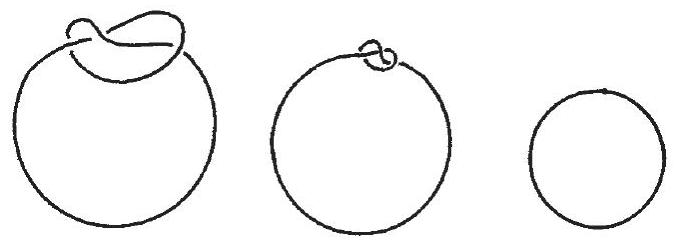
\includegraphics[scale=0.2, center]{2025_05_21_9c06be8de7a55410f8c1g-016}

Figure 1.1. An isotopy of embeddings.

We are going to narrow further the scope of our interest. Topological embeddings $S^{1} \rightarrow S^{3}$ may have a bizarre appearance as Figure 1.2 shows. There is an infinite sequence of similar meshes converging to a limit point $L$ at which this knot is called wild. This example of a wild knot, invented by Fox, indeed has remarkable properties which show that at such a point of wildness something extraordinary may happen. E. Artin and R.H. Fox proved in [114] that the complement of the curve depicted in Figure 1.2 is different from that of a trivial knot. Nevertheless, the knot can obviously be unravelled from the right - at least finitely many stitches can.\\
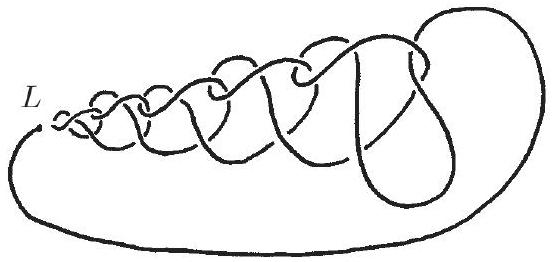
\includegraphics[scale=0.2, center]{2025_05_21_9c06be8de7a55410f8c1g-017}

Figure 1.2. A wild knot.\\

1.3 Definition (Tame knots). 

\begin{DEF}{KNO-B14-02-07}{Zahme und Wilde Knoten}
A knot is called tame if it is ambient isotopic to a piecewise linear embedding in $\mathbb{R}^{3}$ resp. $S^{3}$. A knot is wild if it is not tame.
\end{DEF}

If a knot is tame, any connected proper part $\alpha$ of it is ambient isotopic to a straight segment and therefore the complement $S^{3}-\alpha$ is simply connected. Any proper subarc of the knot of Figure 1.2 which contains the limit point $L$ can be shown [114] to have a non-simply connected complement. From this it appears reasonable to call $L$ a point at which the knot is wild. Wild knots are no exceptions - quite the contrary. J. Milnor proved: "Most" knots are wild [239]. One can even show that almost all knots are wild at every point [42]. Henceforth we shall be concerned only with tame knots. Consequently we shall work always in the p.l.-category (p.l. = piecewise linear). All spaces will be compact polyhedra with a finite simplicial structure, unless otherwise stated. Maps will be piecewise linear. We repeat Definitions 1.1 and 1.2 in an adjusted version:\\


1.4 Definition (p.l.-isotopy and p.l.-ambient isotopy). 

Let $X, Y$ be polyhedra and $f_{0}, f_{1}: X \rightarrow Y$ p.l.-embeddings, $f_{0}$ and $f_{1}$ are p.l.-isotopic if there is a level-preserving p.l.-embedding

$$
F: X \times I \rightarrow Y \times I, F(x, t)=\left(f_{t}(x), t\right), 0 \leq t \leq 1 .
$$

$f_{0}$ and $f_{1}$ are p.l.-ambient isotopic if there is a level-preserving p.l.-isotopy

$$
H: Y \times I \rightarrow Y \times I, H(y, t)=\left(h_{t}(y), t\right),
$$

with $f_{1}=h_{1} f_{0}$ and $h_{0}=\operatorname{id}_{Y}$.\\

In future we shall usually omit the prefix "p.l.".

We are now in a position to give the fundamental definition of a knot as a class of embeddings $S^{1} \rightarrow S^{3}$ resp. $S^{1} \rightarrow \mathbb{R}^{3}$ :\\

1.5 Definition (Equivalence). 

\begin{DEF}{KNO-B14-02-08}{Äquivalenz von (pwl) Knoten}
Two (p.l.)-knots are equivalent if they are (p.l.)-ambient isotopic.
\end{DEF}

We use our terminology loosely in connection with this definition. 

\begin{DEF}{KNO-B14-02-09}{Knoten als Äquivalenzklassen bzgl. Ambient Isotopie}
A knot $\mathfrak{F}$ may be a representative of a class of equivalent knots or the class itself. If the knots $\mathfrak{k}$ and $\mathfrak{k}^{\prime}$ are equivalent, we shall say they are the same, $\mathfrak{k}=\mathfrak{k}^{\prime}$ and use the sign of equality.
\end{DEF}

The main topic of classical knot theory is the classification of knots with regard to equivalence.

Dropping "p.l." defines, of course, a broader field and a more general classification problem. The definition of tame knots (Definition 1.3) suggests applying the Definition 1.2 of "topological" ambient isotopy to define a topological equivalence for this class of knots. At first view one might think that the restriction to the p.l.-category will introduce equivalence classes of a different kind. We shall take up the subject in Chapter 3 to show that this is not true. In fact, two tame knots are topologically equivalent if and only if the p.l.-representatives of their topological classes are p.l-equivalent, see Corollary 3.17.


\subsection{Equivalence of knots}
We defined equivalence of knots by ambient isotopy in the last section. There are different notions of equivalence to be found in the literature which we propose to investigate and compare in this section.

There is a way of defining equivalence of knots which takes advantage of special properties of the embedding space, $\mathbb{R}^{3}$ or $S^{3}$. Fisher [103] proved that an orientation preserving homeomorphism $h: S^{3} \rightarrow S^{3}$ is isotopic to the identity. (A homeomorphism with this property is called a deformation.) We are interested in a special case of Fisher's theorem. We shall prove it with the help of the following theorem which is well known and will not be proved here. See [242, Chapter 17] for a modern account.\\[0pt]

1.6 Theorem (Alexander-Schoenflies [7]). Let $i: S^{2} \rightarrow S^{3}$ be a (p.l.)-embedding. Then

$$
S^{3}=B_{1} \cup B_{2}, i\left(S^{2}\right)=B_{1} \cap B_{2}=\partial B_{1}=\partial B_{2},
$$

where $B_{i}, i=1,2$, is a combinatorial 3-ball ( $B_{i}$ is p.l.-homeomorphic to a 3simplex).

The theorem corresponds to the Jordan curve theorem in dimension two where it holds for topological embeddings. In dimension three it is not true in this generality, Alexander gave a famous example, the Alexander horned sphere [6]. Brown proved in [46] that a for a locally bi-collared ( $n-1$ )-sphere $S$ in $\mathbb{R}^{n}$ there exists an autohomeomorphism of $\mathbb{R}^{n}$ which maps $S$ onto the unit sphere.

We start by proving\\

1.7 Proposition (Alexander-Tietze). Any (p.l.)-homeomorphism $f$ of a (combinatorial) $n$-ball $B$ keeping the boundary fixed is isotopic to the identity by a (p.l.)-ambient isotopy keeping the boundary fixed.

Proof. Define for $(x, t) \in \partial(B \times I)$

$$
H(x, t)= \begin{cases}x & \text { for } t=0 \\ x & \text { for } x \in \partial B \\ f(x) & \text { for } t=1\end{cases}
$$

Every point $(x, t) \in B \times I, t>0$, lies on a straight segment in $B \times I$ joining a fixed interior point $P$ of $B \times 0$ and a variable point $X$ on $\partial(B \times I)$. Extend $H \mid \partial(B \times I)$ linearly on these segments to obtain a (p.l.) level-preserving mapping $H: B \times I \rightarrow$ $B \times I$, in fact, the desired ambient isotopy (Alexander trick, [5], Figure 1.3).\\
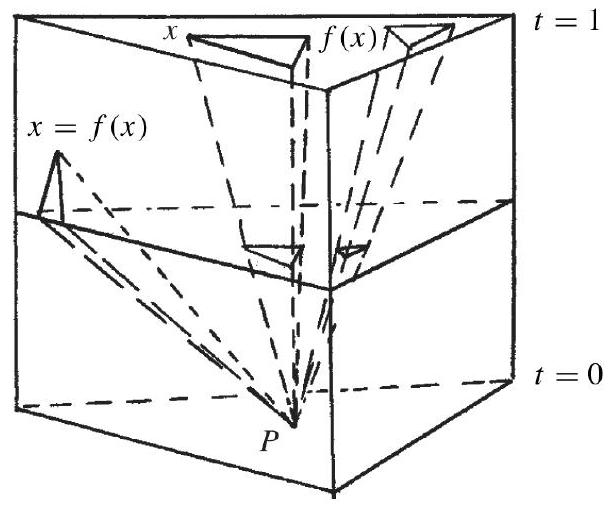
\includegraphics[scale=0.2, center]{2025_05_21_9c06be8de7a55410f8c1g-019}

Figure 1.3. The Alexander trick.

We are now ready to prove the following proposition:\\


1.8 Proposition. 

\begin{PROP}{KNO-B14-02-10}{Äq-Charakterisierung von Äquivalenz von Knoten}
Let $\mathfrak{k}_{0}$ and $\mathfrak{k}_{1}$ be p.l.-knots in $S^{3}$. The following assertions are equivalent:
\begin{enumerate}
  \item There is an orientation-preserving homeomorphism \( f: S^{3} \rightarrow S^{3} \) which carries \( \mathfrak{k}_{0} \) onto \( \mathfrak{k}_{1} \), i.e., \( f \circ \mathfrak{k}_{0} = \mathfrak{k}_{1} \).
  \item \( \mathfrak{K}_{0} \) and \( \mathfrak{K}_{1} \) are equivalent (ambient isotopic).
\end{enumerate}
\end{PROP}


\begin{PROOF}{KNO-B14-02-11}{P: Äq-Charakterisierung von Äquivalenz von Knoten}
Proof. (1) $\Longrightarrow$ (2): We begin by showing that there is an ambient isotopy $H(x, t)=$ $\left(h_{t}(x), t\right)$ of $S^{3}$ such that $h_{1} f$ leaves fixed a 3-simplex $\left[P_{0}, P_{1}, P_{2}, P_{3}\right]$. If $f: S^{3} \rightarrow$ $S^{3}$ has a fixed point, choose it as $P_{0}$; if not, let $P_{0}$ be any interior point of a 3-simplex $\left[s^{3}\right]$ of $S^{3}$. There is an ambient isotopy of $S^{3}$ which leaves $\overline{S^{3}-\left[s^{3}\right]}$ fixed and carries $P_{0}$ over to any other interior point of $\left[s^{3}\right]$. If $\left[s^{3}\right]$ and $\left[s^{\prime 3}\right]$ have a common 2-face, one can easily construct an ambient isotopy moving an interior point $P_{0}$ of $\left[s^{3}\right]$ to an interior point $P_{0}^{\prime}$ of $\left[s^{\prime 3}\right]$ which is the identity outside $\left[s^{3}\right] \cup\left[s^{\prime 3}\right]$ (Figure 1.4).

So there is an ambient isotopy $H^{0}$ with $h_{1}^{0} f\left(P_{0}\right)=P_{0}$, since any two 3 -simplices can be connected by a chain of adjoining ones. Next we choose a point $P_{1} \neq P_{0}$ in\\
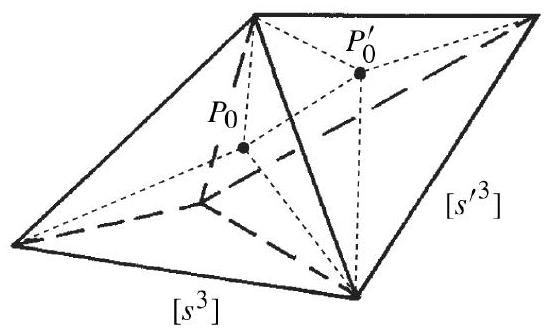
\includegraphics[scale=0.2, center]{2025_05_21_9c06be8de7a55410f8c1g-020}

Figure 1.4\\
the simplex star of $P_{0}$, and by similar arguments we construct an ambient isotopy $H^{1}$ with $h_{1}^{1} h_{1}^{0} f$ leaving fixed the 1 -simplex $\left[P_{0}, P_{1}\right]$. A further step leads to $h_{1}^{2} h_{1}^{1} h_{1}^{0} f$ with a fixed 2-simplex [ $P_{0}, P_{1}, P_{2}$ ]. At this juncture the assumption comes in that $f$ is required to preserve the orientation. A point $P_{3} \notin\left[P_{0}, P_{1}, P_{2}\right]$, but in the star of $\left[P_{0}, P_{1}, P_{2}\right]$ will be mapped by $h_{1}^{2} h_{1}^{1} h_{1}^{0} f$ onto a point $P_{3}^{\prime}$ in the same half-space with regard to the plane spanned by $P_{0}, P_{1}, P_{2}$. This ensures the existence of the final ambient isotopy $H^{3}$ such that $h_{1}^{3} h_{1}^{2} h_{1}^{1} h_{1}^{0} f$ leaves fixed $\left[P_{0}, P_{1}, P_{2}, P_{3}\right]$. The assertion follows from the fact that $H=H^{3} H^{2} H^{1} H^{0}$ is an ambient isotopy, $H(x, t)=$ $\left(h_{t}(x), t\right)$. By Theorem 1.6 the complement of $\left[P_{0}, P_{1}, P_{2}, P_{3}\right]$ is a combinatorial 3-ball and by Theorem 1.7 there is an ambient isotopy which connects $h_{1} f$ with the identity of $S^{3}$.

$(2) \Longrightarrow(1)$ follows from the definition of an ambient isotopy.\\[0pt]
\end{PROOF}


K. Reidemeister [294] gave an elementary introduction into knot theory stressing the combinatorial aspect, which is also the underlying concept of his book "Knotentheorie" [296, 302, 303], the first monograph written in 1932 on the subject. He considered knots as simple closed polygonal curves rather then p.l.-maps. In this context, a polygonal knot $\mathfrak{k}$ is a simple polygonal closed curve i.e. the image of a p.l.-map $S^{1} \rightarrow \mathbb{R}^{3}$. Polygonal knots might be oriented or not. If $S^{1}$ is oriented and if $i: S^{1} \rightarrow S^{3}$ is a knot then the image $\mathfrak{k}=i\left(S^{1}\right)$ inherits an orientation (oriented knot). The notion of equivalence has to be adjusted: two oriented polygonal knots are equivalent if there is an ambient isotopy connecting them which respects the orientation of the knots. Reidemeister introduced an isotopy by moves.\\

1.9 Definition ($\Delta$-move). 

Let $u$ be a straight segment of a polygonal knot $\mathfrak{k}$ in $\mathbb{R}^{3}$ (or $S^{3}$ ), and $D$ a triangle in $\mathbb{R}^{3}, \partial D=u \cup v \cup w, u, v, w$ 1-faces of $D$. If $D \cap \mathfrak{k}=u$, then $\mathfrak{k}^{\prime}=(\mathfrak{k}-u) \cup v \cup w$ defines another polygonal knot. We say $\mathfrak{k}^{\prime}$ results from $\mathfrak{k}$ by a $\Delta$-process or a $\Delta$-move. If $\mathfrak{k}$ is oriented, $\mathfrak{k}^{\prime}$ has to carry the orientation induced by that of $\mathfrak{k}-u$. The inverse process is denoted by $\Delta^{-1}$ (see Figure 1.5).\\
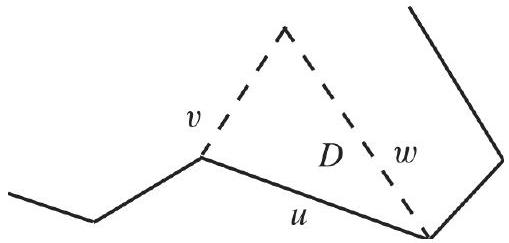
\includegraphics[scale=0.2, center]{2025_05_21_9c06be8de7a55410f8c1g-021}

Figure 1.5. A $\Delta$-move.

Remark: We allow $\Delta$ to degenerate as long as $\mathfrak{k}^{\prime}$ remains simple. This means that $\Delta$ resp. $\Delta^{-1}$ may be a bisection resp. a reduction in dimension one.\\
1.10 Definition (Combinatorial equivalence). Two polygonal knots are combinatorially equivalent or isotopic by moves, if there is a finite sequence of $\Delta$ - and $\Delta^{-1}$-moves that transforms one knot to the other.

1.11 Proposition. 

Let $\mathfrak{k}_{0}$ and $\mathfrak{k}_{1}$ be two polygonal knots in $\mathbb{R}^{3}$. The following assertions are equivalent:\\
(1) There is an orientation preserving homeomorphism $f: S^{3} \rightarrow S^{3}$ which carries $\mathfrak{k}_{0}$ onto $\mathfrak{k}_{1}, f\left(\mathfrak{k}_{0}\right)=\mathfrak{k}_{1}$.\\
(2) $\mathfrak{k}_{0}$ and $\mathfrak{k}_{1}$ are equivalent (ambient isotopic).\\
(3) $\mathfrak{K}_{0}$ and $\mathfrak{K}_{1}$ are combinatorially equivalent (isotopic by moves).

Proof. The equivalence (1) $\Longleftrightarrow$ (2) follows from the proof of Proposition 1.8.\\
Next we prove (1) $\Longrightarrow$ (3): Let $h: S^{3} \rightarrow S^{3}$ be an orientation preserving homeomorphism and $\mathfrak{K}_{1}=h\left(\mathfrak{K}_{0}\right)$. The preceding argument (see the proof of Proposition 1.8) shows that there is another orientation preserving homeomorphism $g: S^{3} \rightarrow S^{3}$, $g\left(\mathfrak{F}_{0}\right)=\mathfrak{F}_{0}$, such that $h g$ leaves fixed some 3 -simplex $\left[s^{3}\right]$ which will have to be chosen outside a regular neighborhood of $\mathfrak{k}_{0}$ and $\mathfrak{k}_{1}$. For an interior point $P$ of $\left[s^{3}\right]$ consider $S^{3}-\{P\}$ as Euclidean 3-space $\mathbb{R}^{3}$. There is a translation $\tau$ of $\mathbb{R}^{3}$, which moves $\mathfrak{K}_{0}$ into $\left[s^{3}\right]-\{P\}$. It is easy to prove that $\mathfrak{K}_{0}$ and $\tau\left(\mathfrak{K}_{0}\right)$ are isotopic by moves (see Figure 1.6). We claim that $\mathfrak{K}_{1}=h g\left(\mathfrak{K}_{0}\right)$ and $h g \tau\left(\mathfrak{K}_{0}\right)=\tau\left(\mathfrak{K}_{0}\right)$ are isotopic by moves also, which would complete the proof. Choose a subdivision of the triangulation of $S^{3}$ such that the triangles used in the isotopy by moves between $\mathfrak{K}_{0}$ and $\tau\left(\mathfrak{K}_{0}\right)$ form a subcomplex of $S^{3}$. There is an isotopy by moves $\mathfrak{F}_{0} \rightarrow \tau\left(\mathfrak{F}_{0}\right)$ which is defined on the triangles of the subdivision. $h g: S^{3} \rightarrow S^{3}$ maps the subcomplex onto another one carrying over the isotopy by moves (see Graeub [139, 140]).\\
$(3) \Longrightarrow(1)$. It is not difficult to construct a homeomorphism of $S^{3}$ onto itself which realizes a $\Delta^{ \pm 1}$-move and leaves fixed the rest of the knot. Choose a regular neighborhood $U$ of the 2 -simplex which defines the $\Delta^{ \pm 1}$-move whose boundary meets the knot at two points. By linear extension one can obtain a homeomorphism producing the $\Delta^{ \pm 1}$-move in $U$ and leaving $S^{3}-U$ fixed.\\
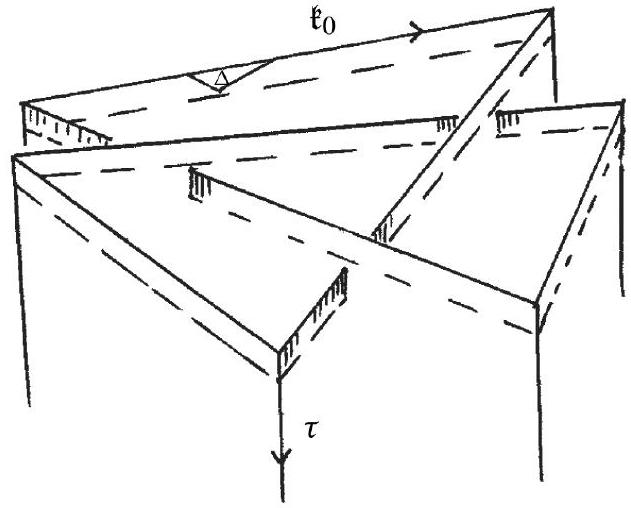
\includegraphics[scale=0.2, center]{2025_05_21_9c06be8de7a55410f8c1g-022}

Figure 1.6. The knots $\mathfrak{k}$ and $\tau(\mathfrak{k})$ are isotopic by $\Delta$-moves.

The image of a p.l.-embedding $i: S^{1} \rightarrow S^{3}$ is a polygonal knot in $S^{3}$ and it follows from Proposition 1.11 that two p.l.-ambient isotopic p.l-embeddings give combinatorially equivalent polygonal knots. Let us investigate to what extent a polygonal knot determines a p.l.-embedding.\\
1.12 Lemma. Let $i: S^{1} \rightarrow S^{3}$ be a p.l.-embedding and denote by $\mathfrak{k}=i\left(S^{1}\right)$ the associated polygonal knot.

If $j: \mathfrak{k} \rightarrow \mathfrak{k}$ is an orientation preserving p.l.-homeomorphism then there exists an orientation preserving homeomorphism $f: S^{3} \rightarrow S^{3}$, supported by a regular neighborhood of $\mathfrak{k}$, such that the restriction of $f \mid \mathfrak{k}$ coincides with $j$.

Proof. Note first that every orientation preserving p.l.-homeomorphism $j: \mathfrak{k} \rightarrow \mathfrak{k}$ is p.l.-ambient isotopic to the identity. More precisely, $j$ is a finite composition of homeomorphism which are supported by a closed arc of $\mathfrak{k}$. This can be proved by following the argument used in the first part of the proof of Proposition 1.8. Therefore it is sufficient to prove the lemma for a homeomorphism $j$ supported by a closed arc $\alpha \subset \mathfrak{k}$.

Let $V=V(\alpha)$ be a regular neighborhood of $\alpha \subset S^{3}$ and define $f$ to be the identity on the complement $S^{3}-V$. Hence, ( $V, \mathfrak{E} \cap V$ ) is an unknotted ball pair and we can extend the identity on the boundary of the ball pair to a homeomorphism which agrees with $j$ on $\mathfrak{k} \cap V$ (see Rourke-Sanderson [311, Prop. 4.4]). This extends $f$ to $V$ such $f \mid \mathfrak{k}=j$.\\
1.13 Corollary. Let $S^{1}$ be oriented and let $i_{1}, i_{2}: S^{1} \rightarrow S^{3}$ be two p.l.-embeddings.

The two oriented polygonal knots $\mathfrak{k}_{1}=i_{1}\left(S^{1}\right)$ and $\mathfrak{k}_{2}=i_{2}\left(S^{1}\right)$ are equivalent if and only if $i_{1}$ and $i_{2}$ are p.l.-ambient isotopic.

Proof. If there exists an orientation preserving homeomorphism $h: S^{3} \rightarrow S^{3}$ such that $h \mid \mathfrak{k}_{1}: \mathfrak{k}_{1} \rightarrow \mathfrak{k}_{2}$ preserves the orientation, then

$$
j=i_{2} \circ i_{1}^{-1} \circ\left(h \mid \mathfrak{k}_{1}\right)^{-1}: \mathfrak{k}_{2} \rightarrow \mathfrak{k}_{2}
$$

is orientation preserving. By Lemma 1.12 there exists an orientation preserving homeomorphism $f: S^{3} \rightarrow S^{3}$ such that $f \mid \mathfrak{k}_{2}=j$ and $(f \circ h) \circ i_{1}=i_{2}$. Hence, Proposition 1.11 implies the assertion of the corollary.

It follows that the isotopy by $\Delta$-moves provides a means to formulate the knot problem on an elementary level. It is also useful as a method in proofs of invariance.

There will be a certain abuse of language in this book to avoid complicating the notation. A knot $\mathfrak{k}$ will be an embedding, a class of embeddings, the image $i\left(S^{1}\right)=\mathfrak{k}$ (a simple polygonal closed curve), or a class of such curves.

\section*{C Knot projections}

\begin{REM}{KNO-B14-02-12}{Setting für Projektion von Knoten}
Geometric description in 3-spaces is complicated. The data that determine a knot are usually given by a projection of $\mathfrak{E}$ onto a plane $E$ (projection plane) in $\mathbb{R}^{3}$. (In this paragraph we prefer $\mathbb{R}^{3}$ with its Euclidean metric to $S^{3}$; a knot $\mathfrak{k}$ will always be thought of as a simple closed polygon in $\mathbb{R}^{3}$.) A point $P \in p(\mathfrak{k}) \subset E$ whose preimage $p^{-1}(P)$ under the projection $p: \mathbb{R}^{3} \rightarrow E$ contains more than one point of $\mathfrak{k}$ is called a multiple point.
\end{REM}


1.14 Definition (Regular projection). 

\begin{DEF}{KNO-B14-02-13}{Reguläre Projektion von Knoten}
A projection $p$ of a knot $\mathfrak{E}$ is called regular if\\
\begin{enumerate}
  \item There are only finitely many multiple points \( \left\{P_{i} \mid 1 \leq i \leq n\right\} \), and all multiple points are double points, that is, \( p^{-1}\left(P_{i}\right) \) contains two points of \( \mathfrak{k} \).
  \item No vertex of \( \mathfrak{k} \) is mapped onto a double point.
\end{enumerate}
\end{DEF}


\begin{DEF}{KNO-B14-02-14}{Ordnung eines Knoten}
The minimal number of double points or crossings $n$ in a regular projection of a knot is called the order of the knot.
\end{DEF} 

A regular projection avoids occurrences as depicted in Figure 1.7.\\
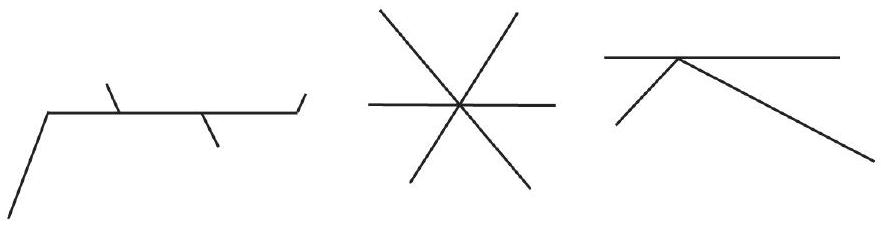
\includegraphics[scale=0.2, center]{2025_05_21_9c06be8de7a55410f8c1g-023}

Figure 1.7. Non-regular projections.\\

There are sufficiently many regular projections.\\

1.15 Proposition. 

\begin{PROP}{KNO-B14-02-15}{Menge der regulären Projektion ist offen und dicht in Menge der Projektionen}
The set of regular projections is open and dense in the space of all projections.
\end{PROP}

\begin{PROOF}{KNO-B14-02-16}{P: Menge der regulären Projektion ist offen und dicht in Menge der Projektionen}
Proof. Think of directed projections as points on a unit sphere $S^{2} \subset \mathbb{R}^{3}$ with the induced topology. A standard argument (general position) shows that singular (nonregular) projections are represented on $S^{2}$ by a finite number of curves. (The reader is referred to Reidemeister [294], Crowell and Fox [80] or Burde [50] for a more detailed treatment.)
\end{PROOF}

\begin{REM}{KNO-B14-02-17}{Rekonstruierbarkeit von Knoten aus regulären Knoten}
The projection of a knot does not determine the knot, but if at every double point in a regular projection the overcrossing line is marked, the knot can be reconstructed from the projection
\end{REM} 

(Figure 1.8).
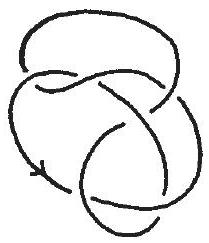
\includegraphics[scale=0.2, center]{2025_05_21_9c06be8de7a55410f8c1g-024}

Figure 1.8


\begin{REM}{KNO-B14-02-18}{Knoten-Projektion / Knoten-Diagramm}
If the knot is oriented, the projection inherits the orientation. The projection of a knot with this additional information is called a knot projection or knot diagram.
\end{REM} 

\begin{DEF}{KNO-B14-02-19}{Äquivalenz von Knoten Diagrammen bzgl Isotopie}
Two knot diagrams will be regarded as equal if they are isotopic in $E$ as graphs, where the isotopy is required to respect overcrossing resp. undercrossing.
\end{DEF} 

Equivalent knots can be described by many different diagrams, but they are connected by simple operations.


1.16 Definition (Reidemeister moves). 

\begin{DEF}{KNO-B14-02-20}{Äquivalenz von Knoten Diagrammen durch Reidemeister Moves}
Two knot diagrams are called equivalent if they are connected by a finite sequence of Reidemeister moves $\Omega_{i}, i=1,2,3$ or their inverses $\Omega_{i}^{-1}$.

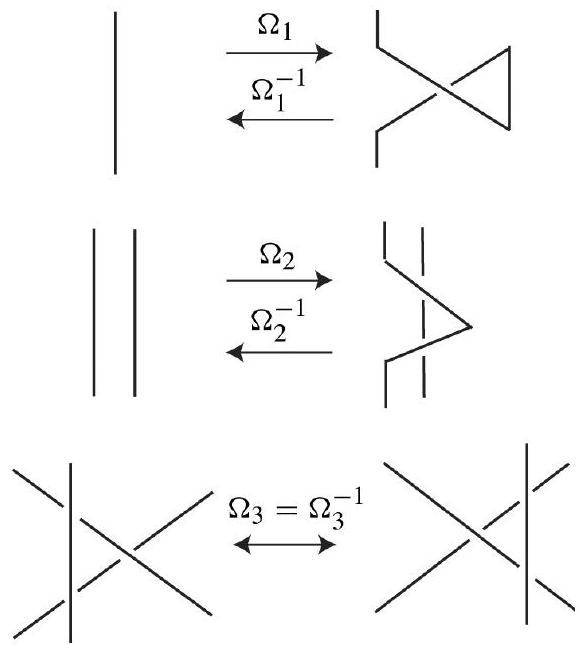
\includegraphics[scale=0.2, center]{2025_05_21_9c06be8de7a55410f8c1g-025(1)}
Figure 1.9. The Reidemeister moves.
\end{DEF}

\begin{REM}{KNO-B14-02-21}{Äquivalente Diagramme definieren äquivalente Knoten}
The operations $\Omega_{i}^{ \pm 1}$ effect local changes in the diagram. Evidently all these operations can be realized by ambient isotopies of the knot; equivalent diagrams therefore define equivalent knots.
\end{REM}

The converse is also true:

1.17 Proposition. 

\begin{PROP}{KNO-B14-02-22}{Äquivalenz von Äquivalenz von Knoten und Äquivalenz der Knoten Diagramme}
Two knots are equivalent if and only if all their diagrams are equivalent.
\end{PROP}

\begin{PROOF}{KNO-B14-02-23}{P: Äquivalenz von Äquivalenz von Knoten und Äquivalenz der Knoten Diagramme}
Proof. The first step in the proof will be to verify that any two regular projections $p_{1}, p_{2}$ of the same simple closed polygon $\mathfrak{k}$ are connected by $\Omega_{i}^{ \pm 1}$-moves. Let $p_{1}, p_{2}$ again be represented by points on $S^{2}$, and choose on $S^{2}$ a polygonal path $s$ from $p_{1}$ to $p_{2}$ in general position with respect to the lines of singular projections on $S^{2}$. When such a line is crossed the diagram will be changed by an operation $\Omega_{i}^{ \pm 1}$, the actual type depending on the type of singularity, see Figure 1.7, corresponding to the line that is crossed.

It remains to show that for a fixed projection equivalent knots possess equivalent diagrams. According to Proposition 1.8 it suffices to show that a $\Delta^{ \pm 1}$-move induces $\Omega_{i}^{ \pm 1}$-operations on the projection. This again is easily verified (Figure 1.10).\\
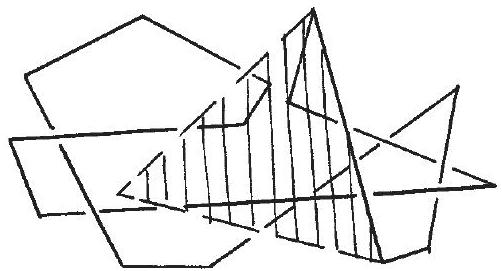
\includegraphics[scale=0.2, center]{2025_05_21_9c06be8de7a55410f8c1g-025}

Figure 1.10\\[0pt]
\end{PROOF}

Proposition 1.17 allows an elementary approach to knot theory. It is possible to continue on this level and define invariants for diagrams with respect to equivalence. The so-called Abbildungsmengen are such invariants which were introduced by G. Burde in 1978 [50]. These invariants became well-known under the name quandles and are now systematically studied (see for example the article by R. Fenn and C. Rourke [99]).

One might be tempted to look for a finite algorithm to decide equivalence of diagrams by establishing an a priori bound for the number of crossings. Such a bound is not known, and a simple counterexample shows that it can at least not be the maximum of the crossings that occur in the diagrams to be compared. The diagram of Figure 1.11\\
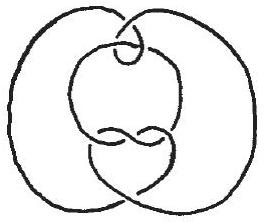
\includegraphics[scale=0.2, center]{2025_05_21_9c06be8de7a55410f8c1g-026}

Figure 1.11\\
is that of a trivial knot, however, on the way to a simple closed projection, via moves $\Omega_{i}^{ \pm 1}$ the number of crossings will increase. This follows from the fact that the diagram only allows operations $\Omega_{1}^{+1}, \Omega_{2}^{+1}$ which increase the number of crossings. Additionally, Figure 1.11 demonstrates: The operations $\Omega_{i}, i=1,2,3$ are "independent" one cannot dispense with any of them (Exercise E 1.5), see Trace [352].

\subsection{Global geometric properties}

In this section we will discuss two theorems (without giving proofs) which connect the property of "knottedness" and "linking" with other geometric properties of the curves in $\mathbb{R}^{3}$. The first is the following theorem of E. Pannwitz [280]:\\
1.18 Theorem (E. Pannwitz). If $\mathfrak{k}$ is a non-trivial knot in $\mathbb{R}^{3}$, then there is a straight line which meets $\mathfrak{k}$ in four points.

If a link of two components $\mathfrak{k}_{i}, i=1,2$, is not splittable, then there is a straight line which meets $\mathfrak{F}_{1}$ and $\mathfrak{F}_{2}$ in two points $A_{1}, B_{1}$ resp. $A_{2}, B_{2}$ each with an ordering $A_{1}, A_{2}, B_{1}, B_{2}$ on the line. (Such a line is called a quadrisecant of $\mathfrak{F}$ ).

It is easy to see that the theorem does not hold for the trivial knot or a splittable linkage. (A link is splittable or split if it can be separated in $\mathbb{R}^{3}$ by a 2 -sphere.)

What E. Pannwitz proved was actually something more general. For any knot $\mathfrak{F} \subset$ $\mathbb{R}^{3}$ there is a singular disk $D \subset \mathbb{R}^{3}$ spanning $\mathfrak{k}$. For example, such a disk can be constructed by erecting a cone over a regular projection of $\mathfrak{k}$ (Figure 1.12). If $D \subset \mathbb{R}^{3}$ is immersed in general position, there will be a finite number of singular points on $\mathfrak{k}$ (boundary singularities).\\
1.19 Definition (Knottedness). The minimal number of boundary singularities of a disk spanning a knot $\mathfrak{k}$ is called the knottedness $k$ of $\mathfrak{k}$.\\
1.20 Theorem (Pannwitz). The knottedness $k$ of a non-trivial knot is an even number. A knot of knottedness $k$ possesses $\frac{k^{2}}{2}$ quadrisecants.

The proof of this theorem - which generalizes the first part of 1.18 - is achieved by cut-and-paste techniques as used in the proof of Dehn's Lemma. (See also J.-P. Otal [278] and G. Kuperberg [205].)





\pagebreak


\section{Geometric concepts}



Some of the charm of knot theory arises from the fact that there is an intuitive geometric approach to it. We shall discuss in this chapter some standard constructions and presentations of knots and various geometric devices connected with them.

\subsection{Geometric properties of projections}

Let $\mathfrak{k}$ be an oriented knot in oriented 3 -space $\mathbb{R}^{3}$.\\

2.1 Definition (Symmetries). 

\begin{DEF}{KNO-B14-02-24}{Invertierung und Spiegelung von Knoten}
The knot obtained from $\mathfrak{k}$ by inverting its orientation is called the inverted knot and denoted by $- \mathfrak{k}$. 

The mirror-image of $\mathfrak{k}$ or mirrored knot is denoted by $\mathfrak{k}^{*}$, it is obtained by a reflection of $\mathfrak{k}$ in a plane.

A knot $\mathfrak{k}$ is called invertible if $\mathfrak{k}=-\mathfrak{k}$, and amphicheiral if $\mathfrak{k}=\mathfrak{k}^{*}$.
\end{DEF}

The trefoil is invertible; the rotation by $\pi$ about the axis indicated in Figure 2.1 (a) is a symmetry which reverses the orientation of the knot. The same holds for the only knot with the minimal number 4 of crossings, the four-knot $4_{1}$ (see Figure 2.1 (c)):

The trefoil was shown to be non-amphicheiral by M. Dehn in 1914 [85, 87]. The right-handed trefoil and its mirror-image, the left-handed trefoil, are displayed in Figure 2.1 (a) and Figure 2.1 (b) respectively. The four-knot is amphicheiral, this property is shown in Figure 2.2. Hence the four-knot $4_{1}$ is both invertible and amphicheiral.\\
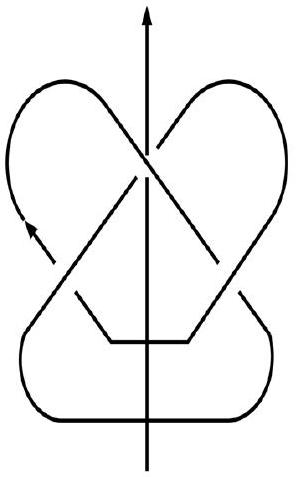
\includegraphics[scale=0.2, center]{2025_05_21_9c06be8de7a55410f8c1g-030}

Figure 2.1 (a). The righthanded trefoil.\\
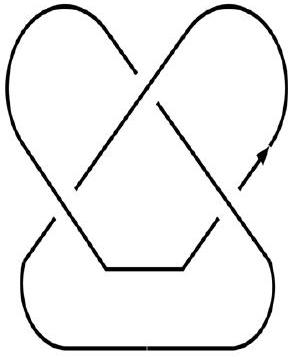
\includegraphics[scale=0.2, center]{2025_05_21_9c06be8de7a55410f8c1g-030(2)}

Figure 2.1 (b). The lefthanded trefoil.\\
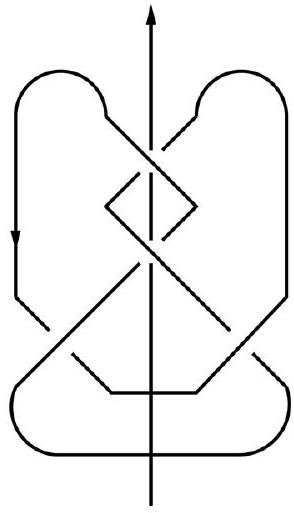
\includegraphics[scale=0.2, center]{2025_05_21_9c06be8de7a55410f8c1g-030(1)}

Figure 2.1 (c). The four-knot.\\
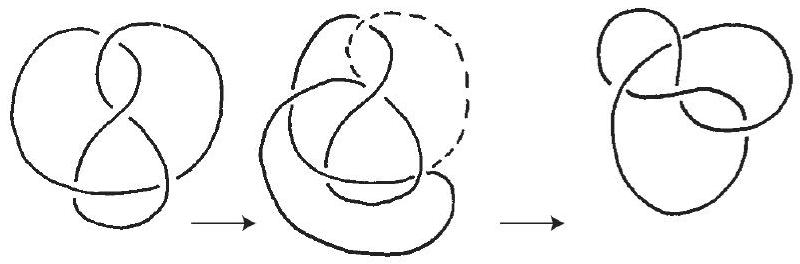
\includegraphics[scale=0.2, center]{2025_05_21_9c06be8de7a55410f8c1g-031(1)}

Figure 2.2. The four-knot is amphicheiral.

The existence of non-invertible knots was proved by H. Trotter [356]. That the knot $8_{17}$ is non-invertible was first proved by A. Kawauchi [189] and independently by F. Bonahon and L. Siebenmann in 1979 [37] using geometric methods. It is the least crossing non-invertible knot, the only one with 8 crossings. Moreover, the knot $\mathfrak{k}=$ $8_{17}$ is negative amphicheiral i.e. $\mathfrak{k}=-\mathfrak{k}^{*}$. By inspection, the rotation by $\pi$ about the axis indicated in Figure 2.3 maps $\mathfrak{k}$ to $-\mathfrak{k}^{*}$.\\
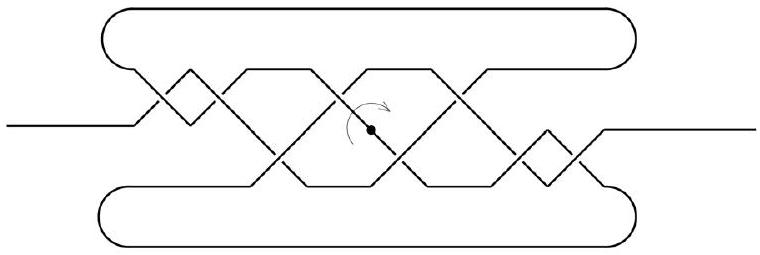
\includegraphics[scale=0.2, center]{2025_05_21_9c06be8de7a55410f8c1g-031}

Figure 2.3 The knot $8_{17}$ is negative amphicheiral.

For this and more refined notions of symmetries in knot theory, see R. Hartley [150], A. Kawauchi [190, Chap. 10] and F. Bonahon and L. Siebenmann [37].\\


2.2 Definition (Alternating knot). 

\begin{DEF}{KNO-B14-02-25}{Alternierende Knoten (Projektion)}
A knot projection is called alternating if uppercrossings and undercrossings alternate while running along the knot. A knot is called alternating if it possesses an alternating projection; otherwise it is non-alternating.
\end{DEF}

The existence of non-alternating knots was first proved by C. Bankwitz [13], see Proposition 13.30.

Alternating projections are frequently printed in knot tables without marking undercrossings. It is an easy exercise to prove that any such projection can be furnished in exactly two ways with undercrossings to become alternating; the two possibilities belong to mirrored knots. Without indicating undercrossings, a closed plane curve does not hold much information about the knot whose projection it might be. Given such a curve there is always a trivial knot that projects onto it. To prove this assertion just choose a curve $\mathfrak{k}$ which ascends monotonically in $\mathbb{R}^{3}$ as one runs along the projection, and close it by a segment in the direction of the projection.\\
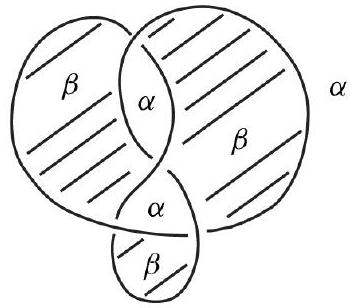
\includegraphics[scale=0.2, center]{2025_05_21_9c06be8de7a55410f8c1g-032(1)}

Figure 2.4. The chessboard coloring.

\begin{REM}{KNO-B14-02-26}{Tessellation der Projektionsfläche}
A finite set of closed plane curves defines a tessellation of the plane by simply connected regions bounded by arcs of the curves, and a single infinite region. (This can be avoided by substituting a 2 -sphere for the plane.) The regions can be colored by two colors like a chessboard such that regions of the same color meet only at double points (Figure 2.4, E 2.2). The proof is easy. If the curve is simple, the fact is well known; if not, omit a simply closed partial curve $s$ and color the regions by an induction hypothesis. Replace $s$ and exchange the coloring for all points inside $s$.
\end{REM}


2.3 Definition (Graph of a knot). 

\begin{DEF}{KNO-B14-02-27}{Graphen eines Knoten}
Let a regular knot diagram be chessboard colored with colors $\alpha$ and $\beta$. Assign to every double point $A$ of the projection an index $\theta(A)= \pm 1$ with respect to the coloring as defined by Figure 2.5. Denote by $\alpha_{i}$, $1 \leq i \leq m$, the $\alpha$-colored regions of a knot diagram. Define a graph $\Gamma$ whose vertices $P_{i}$ correspond to the $\alpha_{i}$, and whose edges $\alpha_{i j}^{k}$ correspond to the double points $A^{k} \in \partial \alpha^{i} \cap \partial \alpha^{j}$, where $\alpha_{i j}^{k}$ joins $P_{i}$ and $P_{j}$ and carries the index $\theta\left(\alpha_{i j}^{k}\right)=\theta\left(A^{k}\right)$.

If $\beta$-regions are used instead of $\alpha$-regions, a different graph is obtained from the regular projection. The Reidemeister moves $\Omega_{i}$ correspond to moves on graphs which can be used to define an equivalence of graphs (compare Definition 1.16 and Proposition 1.17). It is easy to prove (E 2.5) that the two graphs of a projection belonging to $\alpha$ - and $\beta$-regions are equivalent (see [376]). Another Exercise (E 2.3) shows that\\
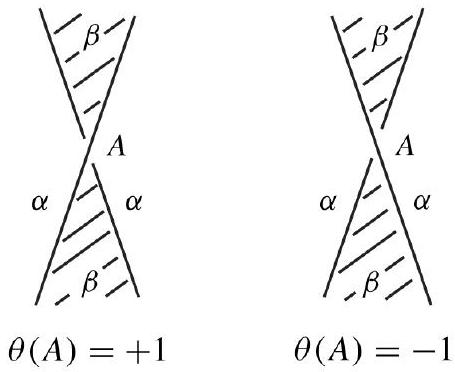
\includegraphics[scale=0.2, center]{2025_05_21_9c06be8de7a55410f8c1g-032}

Figure 2.5. The index $\theta(A)= \pm 1$.\\
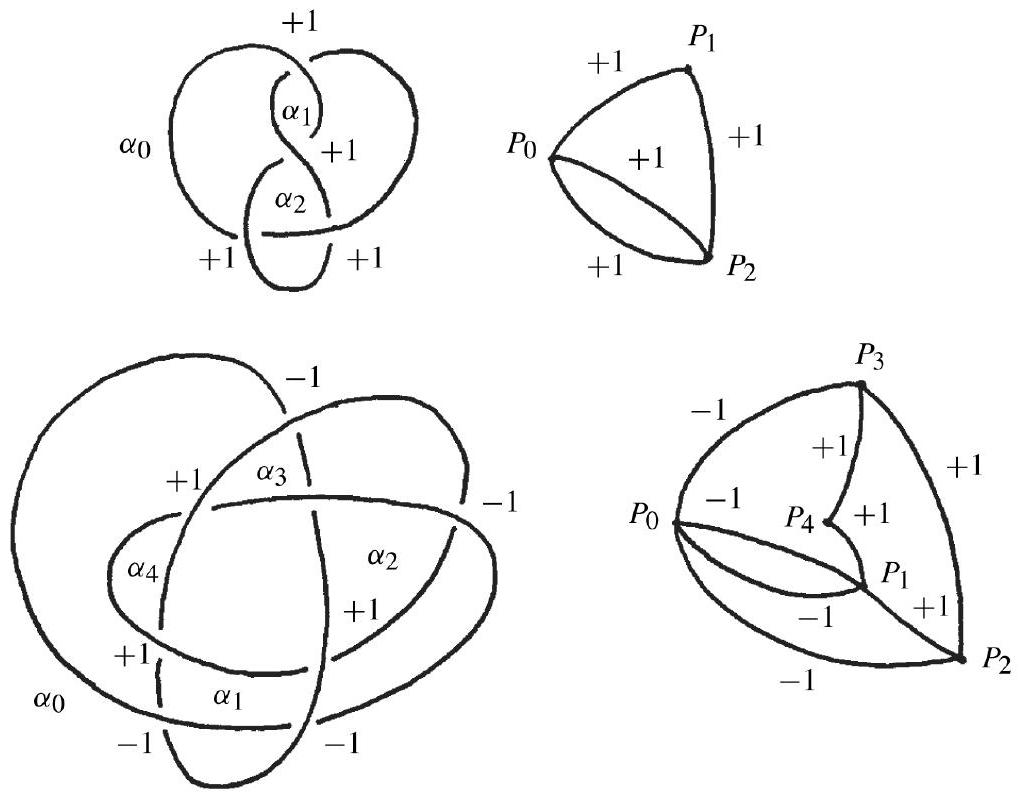
\includegraphics[scale=0.2, center]{2025_05_21_9c06be8de7a55410f8c1g-033}

Figure 2.6\\
a projection is alternating if and only if the index function $\theta(A)$ on the double points is a constant (Figure 2.6).

Graphs of knots have been repeatedly employed in knot theory [12], [76], [196]. We shall take up the subject again in Chapter 13 in connection with the quadratic form of a knot.
\end{DEF}



\subsection{Seifert surfaces and genus}

A geometric fact of some importance is the following:\\

2.4 Proposition (Seifert surface). 

\begin{PROP}{KNO-B14-02-28}{Einfache abgeschlossene orientierte Kurven in $\R^3$ sind Ränder von orientierbaren Flächen}
A simple closed oriented curve $\mathfrak{k} \subset \mathbb{R}^{3}$ is the boundary of an orientable surface $S$, embedded in $\mathbb{R}^{3}$. It is called a Seifert surface of $\mathfrak{k}$.
\end{PROP}

Proof. 

\begin{PROOF}{KNO-B14-02-29}{P: Einfache abgeschlossene orientierte Kurven in $\R3$ sind Ränder von orientierbaren Flächen}
Let $p(\mathfrak{k})$ be a regular projection of $\mathfrak{k}$ equipped with an orientation. By altering $p(\mathfrak{k})$ in the neighborhood of double points as shown in Figure 2.7, $p(\mathfrak{F})$ dissolves into a number of disjoint oriented simple closed curves which are called Seifert cycles. Choose an oriented 2-cell for each Seifert cycle, and embed the 2-cells in $\mathbb{R}^{3}$ as a disjoint union such that their boundaries are projected onto the Seifert cycles. The orientation of a Seifert cycle is to coincide with the orientation induced by the oriented 2-cell.

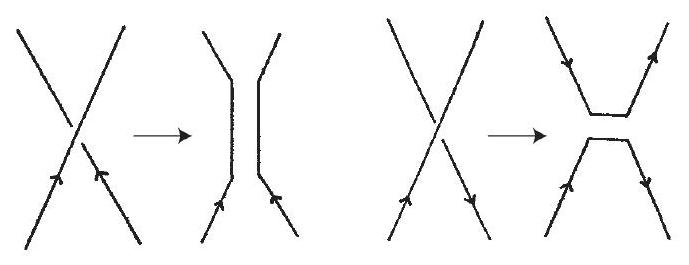
\includegraphics[scale=0.2, center]{2025_05_21_9c06be8de7a55410f8c1g-034}
Figure 2.7

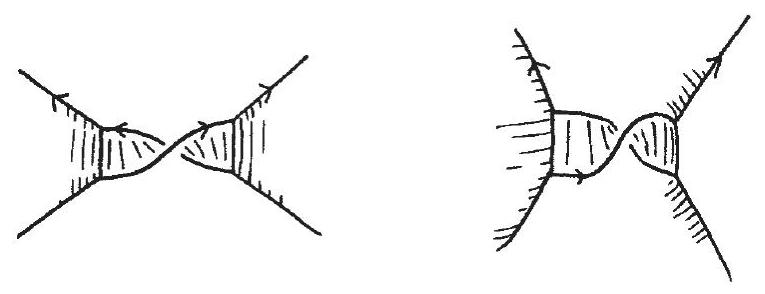
\includegraphics[scale=0.2, center]{2025_05_21_9c06be8de7a55410f8c1g-034(1)}
Figure 2.8

We may place the 2-cells into planes $z=$ const parallel to the projection plane ( $z=0$ ), and choose planes $z=a_{1}, z=a_{2}$ for corresponding Seifert cycles $c_{1}, c_{2}$ with $a_{1}<a_{2}$ if $c_{1}$ contains $c_{2}$. Now we can undo the cut-and-paste-process described in Figure 2.7 by joining the 2-cells at each double point by twisted bands such as to obtain a connected surface $S$ with $\partial S=\mathfrak{k}$ (see Figure 2.8).

Since the oriented 2-cells (including the bands) induce the orientation of $\mathfrak{k}$, they are coherently oriented, and hence, $S$ is orientable.
\end{PROOF}


2.5 Definition (Genus). 

\begin{DEF}{KNO-B14-02-30}{Genus eines Knoten}
The minimal genus $g=g(\mathfrak{k})$ of a Seifert surface spanning a knot $\mathfrak{k}$ is called the genus of the knot $\mathfrak{k}$.
\end{DEF}


\begin{CONC}{KNO-B14-02-31}{Genus eines Knoten als Knoten-Invariante}
Evidently the genus does not depend on the choice of a curve $\mathfrak{k}$ in its equivalence class: If $\mathfrak{k}$ and $\mathfrak{k}^{\prime}$ are equivalent and $S$ spans $\mathfrak{k}$, then there is a homeomorphism $h: S^{3} \rightarrow S^{3}, h(\mathfrak{k})=\mathfrak{k}^{\prime}$ (Proposition 1.5), and $h(S)=S^{\prime}$ spans $\mathfrak{k}^{\prime}$. So the genus $g(\mathfrak{k})$ is a knot invariant, $g(\mathfrak{k})=0$ characterizes the trivial knot, because if $\mathfrak{k}$ bounds a disk $D$ which is embedded in $\mathbb{R}^{3}$ (or $S^{3}$ ), one can use $\Delta$-moves over 2-simplices of $D$ and reduce $\mathfrak{k}$ to the boundary of a single 2 -simplex.
\end{CONC}

The notion of the genus was first introduced by H. Seifert in [328], it holds a central position in knot theory.


The method to construct a Seifert surface by Seifert cycles assigns a surface $S^{\prime}$ of genus $g^{\prime}$ to a given regular projection of a knot. We call $g^{\prime}$ the canonical genus associated with the projection. It is remarkable that in many cases the canonical genus coincides with the (minimal) genus $g$ of the knot. This is always true for alternating projections (Theorem 13.26 (a)). In our table of knot projections up to nine crossings\\
only the projections $8_{20}, 8_{21}, 9_{42}, 9_{44}$ and $9_{45}$ fail to yield $g^{\prime}=g$ : in these cases $g^{\prime}=g+1$.

This was already observed by H. Seifert; the fact that he lists $9_{46}$ instead of $9_{44}$ in [328] is due to the choice of different projections in D. Rolfsen's [309] (and our table) and K. Reidemeister's [296, 302, 303].

There is a general algorithm to determine the genus of a knot due to H. Schubert [321], but its application is complicated. More recently, P. Ozsváth and Z. Szabó [279] showed that knot Floer homology detects the genus of a knot. For other more elementary methods see E 4.11.\\

2.6 Definition and simple properties (Meridian and longitude). 

\begin{CONC}{KNO-B14-02-32}{Meridian und Longitude für tabulare Umgebungen von Knoten}
A tubular neighborhood $V(\mathfrak{k})$ of a knot $\mathfrak{F} \subset S^{3}$ is homeomorphic to a solid torus. There is a simple closed curve $m$ on $\partial V(\mathfrak{f})$ which is null-homologous in $V(\mathfrak{k})$ but not on $\partial V(\mathfrak{k})$; we call $m$ meridian of $\mathfrak{k}$. It is easy to see that any two meridians (if suitably oriented) in $\partial V(\mathfrak{k})$ are isotopic. A Seifert surface $S$ will meet $\partial V(\mathfrak{k})$ in a simple closed curve $\ell$, if $V(\mathfrak{k})$ is suitably chosen: $\ell$ is called a longitude of $\mathfrak{k}$. We shall see later on (Proposition 3.1) that $\ell$, too, is unique up to isotopy on $\partial V(\mathfrak{k})$. If $\mathfrak{k}$ and $S^{3}$ are oriented, we may assign orientations to $m$ and $\ell$ : The longitude $\ell$ is isotopic to $\mathfrak{k}$ in $V(\mathfrak{k})$ and will be oriented as $\mathfrak{k}$. The meridian will be oriented in such a way that its linking number $\operatorname{lk}(m, \mathfrak{k})$ with $\mathfrak{k}$ in $S^{3}$ is +1 or equivalently, its intersection number $\operatorname{int}(m, \ell)$ with $\ell$ is +1 . From this it follows that $\ell$ is not null-homologous on $\partial V(\mathfrak{k})$.
\end{CONC}


\subsection{Companion knots and product knots}
Another important idea was added by H. Schubert in 1949 [317]: the product of knots.\\
2.7 Definition (Product of knots). Let an oriented knot $\mathfrak{k} \subset \mathbb{R}^{3}$ meet a plane $E$ in two points $P$ and $Q$. The arc of from $P$ to $Q$ is closed by an arc in $E$ to obtain a knot $\mathfrak{k}_{1}$; the other arc (from $Q$ to $P$ ) is closed in the same way and so defines a knot $\mathfrak{F}_{2}$. The knot $\mathfrak{F}$ is called the product or composition of $\mathfrak{F}_{1}$ and $\mathfrak{F}_{2}$, and it is denoted by $\mathfrak{k}=\mathfrak{k}_{1} \# \mathfrak{k}_{2}$; see Figure 2.9. The knot $\mathfrak{k}$ is also called a composite knot when both knots $\mathfrak{k}_{1}$ and $\mathfrak{k}_{2}$ are non-trivial. Moreover, $\mathfrak{k}_{1}$ and $\mathfrak{k}_{2}$ are called factors of $\mathfrak{k}$.

It is easy to see that for any given knots $\mathfrak{k}_{1}, \mathfrak{k}_{2}$ the product $\mathfrak{k}=\mathfrak{k}_{1} \# \mathfrak{k}_{2}$ can be constructed; the product will not depend on the choice of representatives or on the plane $E$. A thorough treatment of the subject will be given in Chapter 7.

There are other procedures to construct more complicated knots from simpler ones.\\
2.8 Definition (Companion knot, satellite knot). Let $\widetilde{\mathcal{F}}$ be a knot in a 3-sphere $\widetilde{S}^{3}$ and $\widetilde{V}$ an unknotted solid torus in $\widetilde{S}^{3}$ with $\widetilde{\mathfrak{F}} \subset \widetilde{V} \subset \widetilde{S}^{3}$. Assume that $\widetilde{\mathfrak{F}}$ is not contained in a 3-ball of $\widetilde{V}$. A homeomorphism $h: \widetilde{V} \rightarrow \widehat{V} \subset S^{3}$ onto a tubular neighborhood $\widehat{V}$ of a non-trivial knot $\widehat{\xi} \subset S^{3}$ which maps a meridian of $\widetilde{S}^{3}-\widetilde{V}$ onto a longitude



\pagebreak



\section{Knot groups}

The investigation of the complement of a knot in $\mathbb{R}^{3}$ or $S^{3}$ has been of special interest since the beginnings of knot theory. H. Tietze [350] was the first to prove the existence of non-trivial knots by computing the fundamental group of the complement of the trefoil. He conjectured that two knot types are equal if and only if their complements are homeomorphic. In 1989 C. M. Gordon and J. Luecke [137] finally proved this conjecture - this proof is beyond the scope of this book. In the attempt to classify knot complements, homological methods are not very helpful. The fundamental group, however, is very effective and we will develop methods to present and study it. In particular, we will use it to show that there are non-trivial knots.

\subsection{Homology}

$V=V(\mathfrak{k})$ denotes a tubular neighborhood of the knot $\mathfrak{k}$ and $C=\overline{S^{3}-V}$ is called the complement of the knot. $H_{j}$ will denote the (singular) homology with coefficients in $\mathbb{Z}$.

3.1 Theorem (Homological properties).


\begin{DEF}{KNO-B14-02-33}{Komplement des Knoten}
$V=V(\mathfrak{k})$ denotes a tubular neighborhood of the knot $\mathfrak{k}$ and $C=\overline{S^{3}-V}$ is called the complement of the knot. $H_{j}$ will denote the (singular) homology with coefficients in $\mathbb{Z}$.
\end{DEF}



\begin{PROP}{KNO-B14-04-03}{Homologie des Knotenkomplements}
Let \( C = \overline{S^3 \setminus V} \) be the complement of the knot. We consider singular homology with integer coefficients, i.e., \( H_j = H_j(-; \mathbb{Z}) \). Then:
\[
H_j(C) \cong
\begin{cases}
\mathbb{Z} & \text{if } j = 0 \text{ or } j = 1, \\
0 & \text{otherwise}.
\end{cases}
\]
\end{PROP}

Proof.

\begin{PROOF}{KNO-B14-04-04}{Homologie des Knotenkomplements}
Here we present one based on homological methods. We use the following well-known results:
$$
H_{n}\left(S^{3}\right)= \begin{cases}\mathbb{Z} & \text { for } n=0,3 \\ 0 & \text { otherwise }\end{cases}
$$
$$
\begin{aligned}
H_{n}(\partial V) & = \begin{cases}\mathbb{Z} & \text { for } n=0,2 \\
\mathbb{Z} \oplus \mathbb{Z} & \text { for } n=1, \\
0 & \text { otherwise, }\end{cases} \\
H_{n}(V)=H_{n}\left(S^{1}\right)= & \begin{cases}\mathbb{Z} & \text { for } n=0,1, \\
0 & \text { otherwise; }\end{cases}
\end{aligned}
$$
they can be found in standard books on algebraic topology, see Spanier [341], StöckerZieschang [346], Hatcher [157].

Since $C$ is connected, $H_{0}(C)=\mathbb{Z}$. For further calculations we use the MayerVietoris sequence of the pair ( $V, C$ ) where $V \cup C=S^{3}, V \cap C=\partial V$ :
\[
\begin{tikzcd}[row sep=small, column sep=small]
H_3(\partial V) \arrow[r] \arrow[d, equal] 
  & H_3(V) \arrow[r, phantom, "\oplus"] \arrow[d, equal] 
  & H_3(C) \arrow[r] 
  & H_3(S^3) \arrow[r] \arrow[d, "\cong", "\mathbb{Z}"']
  & H_2(\partial V) \arrow[r] \arrow[d, "\cong", "\mathbb{Z}"'] 
  & {} \\
0 & 0 & {} & \mathbb{Z} & \mathbb{Z} & {}
\end{tikzcd}
\]

\[
\begin{tikzcd}[row sep=small, column sep=small]
{} \arrow[r]
  & H_2(V) \arrow[r, phantom, "\oplus"] \arrow[d, equal]
  & H_2(C) \arrow[r] 
  & H_2(S^3) \arrow[r] \arrow[d, equal]
  & H_1(\partial V) \arrow[r] \arrow[d, "\cong"]
  & {} \\
{} & 0 & {}& 0 & \mathbb{Z} \oplus \mathbb{Z} & {}
\end{tikzcd}
\]

\[
\begin{tikzcd}[row sep=small, column sep=small]
{} \arrow[r] 
  & H_1(V) \arrow[r, phantom, "\oplus"] \arrow[d, "\cong"] & H_1(C) \arrow[r]
  & H_1(S^3) \arrow[d, equal] \\
{} & \mathbb{Z} & {} & 0
\end{tikzcd}
\]
It follows that $H_{1}(C)=\mathbb{Z}$. Since $\partial V$ is the boundary of the orientable compact 3manifold $C$, the group $H_{2}(\partial V)$ is mapped by the inclusion $\partial V \hookrightarrow C$ to $0 \in H_{2}(C)$. This implies that $H_{2}(C)=0$ and that $H_{3}\left(S^{3}\right) \rightarrow H_{2}(\partial V)$ is surjective; hence, $H_{3}(C)=0$.


Since $C$ is a 3-manifold it follows that $H_{n}(C)=0$ for $n>3$; this is also a consequence of the Mayer-Vietoris sequence.
\end{PROOF}




\begin{PROP}{KNO-B14-04-01}{Homologische Eigenschaften von tabuieren Umgebungen von Knoten}
$V=V(\mathfrak{k})$ denotes a tubular neighborhood of the knot $\mathfrak{k}$ and $C=\overline{S^{3}-V}$ is called the complement of the knot. $H_{j}$ will denote the (singular) homology with coefficients in $\mathbb{Z}$.

\begin{itemize}
  \item[(a)] \( H_{0}(C) \cong H_{1}(C) \cong \mathbb{Z}, \quad H_{n}(C) = 0 \) for \( n \geq 2 \).
  
  \item[(b)] There are two simple closed curves \( m \) and \( \ell \) on \( \partial V \) with the following properties:
  \begin{enumerate}
    \item \( m \) and \( \ell \) intersect in one point,
    \item \( m \sim 0 \), \( \ell \sim \mathfrak{k} \) in \( V(\mathfrak{k}) \),
    \item \( \ell \sim 0 \) in \( C = \overline{S^{3} - V(\mathfrak{k})} \),
    \item \( \operatorname{lk}(m, \mathfrak{k}) = 1 \) and \( \operatorname{lk}(\ell, \mathfrak{k}) = 0 \) in \( S^{3} \).
  \end{enumerate}
\end{itemize}

These properties determine $m$ and $\ell$ up to isotopy on $\partial V(\mathfrak{k})$. We call $m$ a meridian and $\ell$ a longitude of the knot $\mathfrak{k}$. The knot $\mathfrak{k}$ and the longitude $\ell$ bound an annulus $A \subset V$.
\end{PROP}

Proof. 

\begin{PROOF}{KNO-B14-04-02}{P: Homologische Eigenschaften von tabuieren Umgebungen von Knoten}
For (a) there are several proofs. Here we present one based on homological methods. We use the following well-known results:

$$
H_{n}\left(S^{3}\right)= \begin{cases}\mathbb{Z} & \text { for } n=0,3 \\ 0 & \text { otherwise }\end{cases}
$$

$$
\begin{aligned}
H_{n}(\partial V) & = \begin{cases}\mathbb{Z} & \text { for } n=0,2 \\
\mathbb{Z} \oplus \mathbb{Z} & \text { for } n=1, \\
0 & \text { otherwise, }\end{cases} \\
H_{n}(V)=H_{n}\left(S^{1}\right)= & \begin{cases}\mathbb{Z} & \text { for } n=0,1, \\
0 & \text { otherwise; }\end{cases}
\end{aligned}
$$
they can be found in standard books on algebraic topology, see Spanier [341], StöckerZieschang [346], Hatcher [157].

Since $C$ is connected, $H_{0}(C)=\mathbb{Z}$. For further calculations we use the MayerVietoris sequence of the pair ( $V, C$ ) where $V \cup C=S^{3}, V \cap C=\partial V$ :

\[
\begin{tikzcd}[row sep=small, column sep=small]
H_3(\partial V) \arrow[r] \arrow[d, equal] 
  & H_3(V) \arrow[r, phantom, "\oplus"] \arrow[d, equal] 
  & H_3(C) \arrow[r] 
  & H_3(S^3) \arrow[r] \arrow[d, "\cong", "\mathbb{Z}"']
  & H_2(\partial V) \arrow[r] \arrow[d, "\cong", "\mathbb{Z}"'] 
  & {} \\
0 & 0 & {} & \mathbb{Z} & \mathbb{Z} & {}
\end{tikzcd}
\]

\[
\begin{tikzcd}[row sep=small, column sep=small]
{} \arrow[r]
  & H_2(V) \arrow[r, phantom, "\oplus"] \arrow[d, equal]
  & H_2(C) \arrow[r] 
  & H_2(S^3) \arrow[r] \arrow[d, equal]
  & H_1(\partial V) \arrow[r] \arrow[d, "\cong"]
  & {} \\
{} & 0 & {}& 0 & \mathbb{Z} \oplus \mathbb{Z} & {}
\end{tikzcd}
\]

\[
\begin{tikzcd}[row sep=small, column sep=small]
{} \arrow[r] 
  & H_1(V) \arrow[r, phantom, "\oplus"] \arrow[d, "\cong"] & H_1(C) \arrow[r]
  & H_1(S^3) \arrow[d, equal] \\
{} & \mathbb{Z} & {} & 0
\end{tikzcd}
\]
It follows that $H_{1}(C)=\mathbb{Z}$. Since $\partial V$ is the boundary of the orientable compact 3manifold $C$, the group $H_{2}(\partial V)$ is mapped by the inclusion $\partial V \hookrightarrow C$ to $0 \in H_{2}(C)$. This implies that $H_{2}(C)=0$ and that $H_{3}\left(S^{3}\right) \rightarrow H_{2}(\partial V)$ is surjective; hence, $H_{3}(C)=0$.


Since $C$ is a 3-manifold it follows that $H_{n}(C)=0$ for $n>3$; this is also a consequence of the Mayer-Vietoris sequence.

Consider the isomorphism
$$
\mathbb{Z} \oplus \mathbb{Z} \cong H_{1}(\partial V) \rightarrow H_{1}(V) \oplus H_{1}(C)
$$
in the Mayer-Vietoris sequence. The generators of $H_{1}(V) \cong \mathbb{Z}$ and $H_{1}(C) \cong \mathbb{Z}$ are determined up to their inverses. Choose the homology class of $\mathfrak{k}$ as a generator of $H_{1}(V)$ and represent it by a simple closed curve $\ell$ on $\partial V$ which is homologous to 0 in $H_{1}(C)$. These conditions determine the homology class of $\ell$ in $\partial V$; hence, $\ell$ is unique up to isotopy on $\partial V$. A generator of $H_{1}(C)$ can be represented by a curve $m$ on $\partial V$ that is homologous to 0 in $V$. The curves $\ell$ and $m$ determine a system of generators of $H_{1}(\partial V) \cong \mathbb{Z} \oplus \mathbb{Z}$. By a well-known result, we may assume that $m$ is simple and intersects $\ell$ in one point, see e.g. Stillwell [345, 6.4.3], Zieschang, Vogt and Coldewey [382, E 3.22]. As $m$ is homologous to 0 in $V$ it is null-homotopic in $V$, bounds a disk, and is a meridian of the solid torus $V$. The linking number of $m$ and $\mathfrak{F}$ is 1 or -1. If necessary we reverse the direction of $m$ to get (4). These properties determine $m$ up to an isotopy of $\partial V$. A consequence is that $\ell$ and $\mathfrak{k}$ bound an annulus $A \subset V$.

Since $\ell \sim 0$ in $C, \ell$ bounds a surface, possibly with singularities, in $C$. (As we already know, see Proposition 2.4, $\ell$ even spans a surface without singularities: a Seifert surface.)
\end{PROOF}




Theorem 3.1 can be generalized to links (E 3.2). The negative aspect of the theorem is that complements of knots cannot be distinguished by their homological properties.\\



3.2 On the characterization of longitudes and meridians by the complement of a knot. 

With respect to the complement $C$ of a knot, the longitude $\ell$ and the meridian $m$ have quite different properties: The longitude $\ell$ is determined up to isotopy and orientation by $C$; this follows from the fact that $\ell$ is a simple closed curve on $\partial C$ which is not homologous to 0 on $\partial C$ but homologous to 0 in $C$. The meridian $m$ is a simple closed curve on $\partial C$ that intersects $\ell$ at one point; hence, $\ell$ and $m$ represent generators of $H_{1}(\partial C) \cong \mathbb{Z}^{2}$. The meridian is not determined by $C$ because simple closed curves on $\partial C$ which are homologous to $m^{ \pm 1} \ell^{r}, r \in \mathbb{Z}$, have the same properties (see E 3.3).



\pagebreak

\subsection{Wirtinger presentation}

The most important and effective invariant of a knot $\mathfrak{k}$ (or link) is its group: the fundamental group of its complement $\mathfrak{G}=\pi_{1}\left(S^{3}-\mathfrak{k}\right)$. Frequently $S^{3}-\mathfrak{k}$ is replaced by $\mathbb{R}^{3}-\mathfrak{k}$ or by $\overline{S^{3}-V(\mathfrak{k})}$ or $\overline{\mathbb{R}^{3}-V(\mathfrak{k})}$, respectively. The fundamental groups of these various spaces are obviously isomorphic, the isomorphisms being induced by inclusion. There is a simple procedure, due to Wirtinger, to obtain a presentation of a knot group.\\

3.3. 



\begin{CONC}{KNO-B14-03-06}{Wirtinger Prozedur}
Embed the knot $\mathfrak{k}$ into $\mathbb{R}^{3}$ such that its projection onto the plane $\mathbb{R}^{2}$ is regular. The projecting cylinder $Z$ has self-intersections in $n$ projecting rays $a_{i}$ corresponding to the $n$ double points of the regular projection. The $a_{i}$ decompose $Z$ into $n$ 2-cells $Z_{i}$ (see Figure 3.1) where $Z_{i}$ is bounded by $a_{i-1}, a_{i}$ and the overcrossing arc $\sigma_{i}$ of $\mathfrak{k}$.

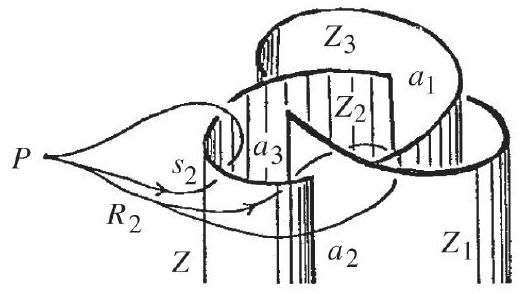
\includegraphics[scale=0.2, center]{2025_05_21_9c06be8de7a55410f8c1g-046}
Figure 3.1

Choose the orientation of $Z_{i}$ to induce on $\sigma_{i}$ the direction of $\mathfrak{k}$. The complement of $Z$ can be retracted parallel to the rays onto a half-space above the knot; thus it is contractible.

To compute $\pi_{1} C$ for some basepoint $P \in C$ observe that there is (up to a homotopy fixing $P$ ) exactly one polygonal closed path in general position relative to $Z$ which intersects a given $Z_{i}$ with intersection number $\varepsilon_{i}$ and which does not intersect the other $Z_{j}$. Paths of this type, taken for $i=1,2, \ldots, n$ and $\varepsilon_{i}=1$, represent generators $s_{i} \in \pi_{1} C$. To see this, let a path in general position with respect to $Z$ represent an arbitrary element of $\pi_{1} C$. Move its intersection points with $Z_{i}$ into the intersection of the curves $s_{i}$. Now the assertion follows since the complement of $Z$ is contractible. Running through an arbitrary closed polygonal path $\omega$ yields the homotopy class as a word $w\left(s_{i}\right)=s_{i_{1}}^{\varepsilon_{1}} \ldots s_{i_{r}}^{\varepsilon_{r}}$ if in turn each intersection with $Z_{i_{j}}$ and intersection number $\varepsilon_{j}$ is put down by writing $s_{i_{j}}^{\varepsilon_{j}}$.

To obtain relations, consider a small path $\varrho_{j}$ in $C$ encircling $a_{j}$ and join it with $P$ by an arc $\lambda_{j}$. Then $\lambda_{j} \varrho_{j} \lambda_{j}^{-1}$ is contractible and the corresponding word $l_{j} r_{j} l_{j}^{-1}$ in the generators $s_{i}$ is a relation. The word $r_{j}\left(s_{j}\right)$ can easily be read off from the knot projection. According to the characteristic $\eta \in\{1,-1\}$ of a double point, see Figure 3.2, we get the relation

$$
r_{j}=s_{j} s_{i}^{-\eta_{j}} s_{k}^{-1} s_{i}^{\eta_{j}} .
$$

\begin{center}
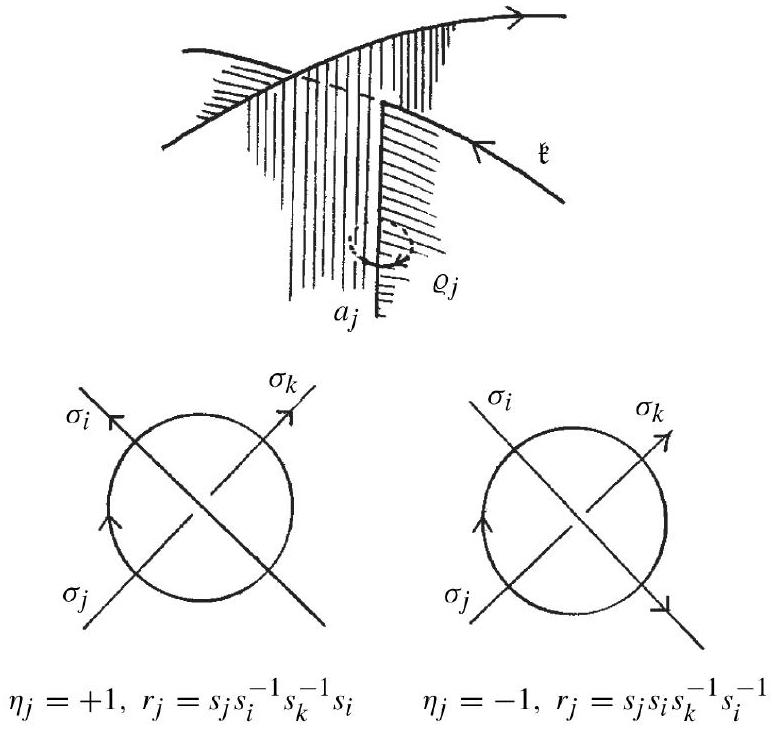
\includegraphics[scale=0.2]{2025_05_21_9c06be8de7a55410f8c1g-047}
\end{center}
Figure 3.2. The Wirtinger relations.
\end{CONC}


3.4 Theorem (Wirtinger presentation). 

\begin{THEO}{KNO-B14-03-01}{Wirtinger Presentation}
Let $\sigma_{i}, i=1,2, \ldots, n$, be the overcrossing arcs of a regular projection of a knot (or link) $\mathfrak{k}$. Then the knot group admits the following so-called Wirtinger presentation:
$$
\mathfrak{G}=\pi_{1}\left(\overline{S^{3}-V(\mathfrak{k})}\right)=\left\langle s_{1}, \ldots, s_{n} \mid r_{1}, \ldots, r_{n}\right\rangle .
$$
The arc $\sigma_{i}$ corresponds to the generator $s_{i}$; a crossing of characteristic $\eta_{j}$ as in Figure 3.2 gives rise to the defining relations
$$
r_{j}=s_{j} s_{i}^{-\eta_{j}} s_{k}^{-1} s_{i}^{\eta_{j}} .
$$
\end{THEO}


Proof. 

\begin{PROOF}{KNO-B14-03-02}{P: Wirtinger Presentation}
It remains to check that $r_{1}, \ldots, r_{n}$ are defining relations. Consider $\mathbb{R}^{3}$ as a simplicial complex $\Sigma$ containing $Z$ as a subcomplex, and denote by $\Sigma^{*}$ the dual complex. Let $\omega$ be a contractible curve in $C$, starting at a vertex $P$ of $\Sigma^{*}$. By simplicial approximation $\omega$ can be replaced by a path in the 1 -skeleton of $\Sigma^{*}$ and the contractible homotopy by a series of homotopy moves which replace arcs on the boundary of 2-cells $\sigma^{2}$ of $\Sigma^{*}$ by the inverse of the rest. If $\sigma^{2} \cap Z=\emptyset$ the deformation over $\sigma^{2}$ has no effect on the words $\omega\left(s_{i}\right)$. If $\sigma^{2}$ meets $Z$ in an arc then the deformation over $\sigma^{2}$ either cancels or inserts a word $s_{i}^{\varepsilon} s_{i}^{-\varepsilon}, \varepsilon \in\{1,-1\}$, in $\omega\left(s_{i}\right)$; hence, it does not affect the element of $\pi_{1} C$ represented by $\omega$. If $\sigma^{2}$ intersects a double line $a_{j}$ then the deformation over $\sigma^{2}$ omits or inserts a relation: a conjugate of $r_{j}$ or $r_{j}^{-1}$ for some $j$.
\end{PROOF}

In the case of a link $\mathfrak{k}$ of $\mu$ components the relations ensure that generators $s_{i}$ and $s_{j}$ are conjugate if the corresponding arcs $\sigma_{i}$ and $\sigma_{j}$ belong to the same component. By abelianizing $\mathfrak{G}=\pi_{1}\left(S^{3}-\mathfrak{k}\right)$ we obtain from Theorem 3.4, see also E 3.2:\\

3.5 Proposition. $H_{1}\left(S^{3}-\mathfrak{k}\right) \cong \mathbb{Z}^{\mu}$ where $\mu$ is the number of components of $\mathfrak{k}$.

Using Proposition 3.5 and duality theorems for homology and cohomology one can calculate the other homology groups of $S^{3}-\mathfrak{k}$, see E 3.2 :\\


3.6 Corollary. 

\begin{KORO}{KNO-B14-03-03}{Relationen der Wirtinger Präsentation sind Konsequenz der anderen Relationen}
Let $\mathfrak{k}$ be a knot or link and $\left\langle s_{1}, \ldots, s_{n} \mid r_{1}, \ldots, r_{n}\right\rangle$ a Wirtinger presentation of $\mathfrak{G}$. Then each defining relation $r_{j}$ is a consequence of the other defining relations $r_{i}, i \neq j$.
\end{KORO}

Proof. 

\begin{PROOF}{KNO-B14-03-07}{P: Relationen der Wirtinger Präsentation sind Konsequenz der anderen Relationen}
Choose the curves $\lambda_{j} \varrho_{j} \lambda_{j}^{-1}$ (see the paragraph before Theorem 3.4) in a plane $E$ parallel to the projection plane and "far down" such that $E$ intersects all $a_{i}$. Let $\delta$ be a disk in $E$ such that $\mathfrak{k}$ is projected into $\delta$, and let $\gamma$ be the boundary of $\delta$. We assume that $P$ is on $\gamma$ and that the $\lambda_{j}$ have only the basepoint $P$ in common. Then, see Figure 3.3,
$$
\gamma \simeq \prod_{j=1}^{n} \lambda_{j} \varrho_{j} \lambda_{j}^{-1} \quad \text { in } E-\left(\bigcup_{j} a_{j} \cap E\right)
$$
\begin{center}
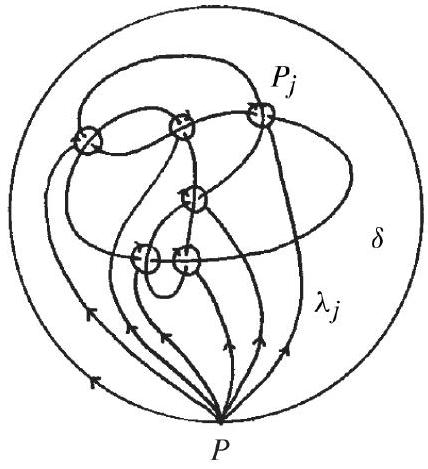
\includegraphics[scale=0.2]{2025_05_21_9c06be8de7a55410f8c1g-049}
\end{center}
Figure 3.3

This implies the equation
$$
1 \equiv \prod_{j=1}^{n} l_{j} r_{j} l_{j}^{-1}
$$
in the free group generated by the $s_{i}$, where $l_{j}$ is the word which corresponds to $\lambda_{j}$. Thus each relation $r_{j}$ is a consequence of the other relations.
\end{PROOF}



3.7 Example (Trefoil knot = clover leaf knot). 

\begin{EXA}{KNO-B14-03-08}{Trefoil knot = clover leaf knot}
From Figure 3.4 we obtain Wirtinger generators $s_{1}, s_{2}, s_{3}$ and defining relations
$$
\begin{array}{ll}
s_{1} s_{2} s_{3}^{-1} s_{2}^{-1} & \text { at the vertex } A, \\
s_{2} s_{3} s_{1}^{-1} s_{3}^{-1} & \text { at the vertex } B, \\
s_{3} s_{1} s_{2}^{-1} s_{1}^{-1} & \text { at the vertex } C .
\end{array}
$$

\begin{center}
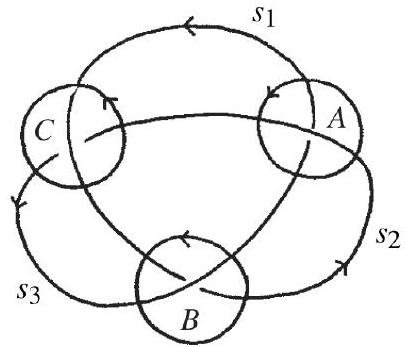
\includegraphics[scale=0.2]{2025_05_21_9c06be8de7a55410f8c1g-049(1)}
\end{center}
Figure 3.4. The Wirtinger relations for the trefoil knot.

Since by Corollary 3.6 one relation is a consequence of the other two, the knot group has the presentation
$$
\begin{aligned}
\left\langle s_{1}, s_{2}, s_{3} \mid s_{1} s_{2} s_{3}^{-1} s_{2}^{-1}, s_{3} s_{1} s_{2}^{-1} s_{1}^{-1}\right\rangle & =\left\langle s_{1}, s_{2} \mid s_{1} s_{2} s_{1} s_{2}^{-1} s_{1}^{-1} s_{2}^{-1}\right\rangle \\
& =\left\langle x, y \mid x^{3}=y^{2}\right\rangle
\end{aligned}
$$

where $y=s_{2} s_{1} s_{2}$ and $x=s_{1} s_{2}$. This group is not isomorphic to $\mathbb{Z}$, since the last presentation shows that it is a free product with amalgamated subgroup $\mathfrak{A}_{1} * \mathfrak{B}_{2}$ where $\mathfrak{A}_{i} \cong \mathbb{Z}$ and $\mathfrak{B}=\left\langle x^{3}\right\rangle=\langle y\rangle$ with $\mathfrak{B} \subsetneq \mathfrak{A}_{i}$. Hence, it is not commutative. This can also be shown directly using the representation $\rho:(\mathcal{G}) \rightarrow \mathrm{SL}_{2}(\mathbb{Z})$ given by

$$
\rho: x \mapsto A=\left(\begin{array}{cc}
0 & 1 \\
-1 & 1
\end{array}\right), \quad \rho: y \mapsto B=\left(\begin{array}{rr}
0 & 1 \\
-1 & 0
\end{array}\right)
$$

since

$$
A \cdot B=\left(\begin{array}{rr}
-1 & 0 \\
-1 & -1
\end{array}\right) \neq\left(\begin{array}{cc}
-1 & 1 \\
0 & -1
\end{array}\right)=B \cdot A
$$

The reader should note that here for the first time in this book the existence of non-trivial knots has been proved, since the group of the trivial knot is cyclic.
\end{EXA}



\begin{REM}{KNO-B14-03-09}{Anmerkung zur Analyse der Fundamentalgruppe des Komplementraumes}
We can approach the analysis of the group of the trefoil knot in a different manner by calculating its commutator subgroup using the Reidemeister-Schreier method. It turns out that $\mathscr{F}^{\prime}$ is a free group of rank 2 , see E 4.2 . We will use this method in the next example.
\end{REM}



3.8 Example (Four-knot or figure-eight knot, Figure 3.5).

\begin{REM}{KNO-B14-03-10}{Four-knot or figure-eight knot}
$$
\begin{aligned}
\mathbb{G}= & \left\langle s_{1}, s_{2}, s_{3}, s_{4} \mid s_{3} s_{4}^{-1} s_{3}^{-1} s_{1}, s_{1} s_{2}^{-1} s_{1}^{-1} s_{3}, s_{4} s_{2}^{-1} s_{3}^{-1} s_{2}\right\rangle \\
= & \left\langle s_{1}, s_{3} \mid s_{3}^{-1} s_{1} s_{3} s_{1}^{-1} s_{3} s_{1}^{-1} s_{3} s_{1}^{-1}\right\rangle \\
= & \left\langle s, u \mid u^{-1} s u s^{-1} u^{-2} s^{-1} u s\right\rangle \\
& \quad \text { where } s=s_{1} \text { and } u=s_{1}^{-1} s_{3}
\end{aligned}
$$

The abelianizing homomorphism $\mathfrak{G} \rightarrow \mathbb{Z}$ maps $s_{i}$ onto 1 which is a generator of $\mathbb{Z}$ and $u$ onto 0 . Hence, $\left\{s^{n} \mid n \in \mathbb{Z}\right\}$ is a system of coset representatives and $\left\{ x_n = s^n u s^{-n} \,\middle|\, n \in \mathbb{Z} \right\}$ the corresponding system of Schreier generators for the commutator subgroup $\left(\mathscr{F}'\right) \quad \text{(see [382, 2.2])}$. The defining relations are

$$
r_{n}=s^{n}\left(u^{-1} s u s^{-1} u^{-2} s^{-1} u s\right) s^{-n}=x_{n}^{-1} x_{n+1} x_{n}^{-2} x_{n-1}, n \in \mathbb{Z} .
$$

\begin{center}
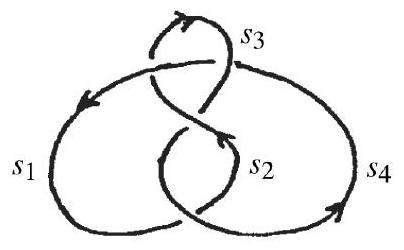
\includegraphics[scale=0.2]{2025_05_21_9c06be8de7a55410f8c1g-050}
\end{center}

Figure 3.5. The figure-eight knot.

Using $r_{1}$, we obtain

$$
x_{2}=x_{1} x_{0}^{-1} x_{1}^{+2} ;
$$

hence, we may drop the generator $x_{2}$ and the relation $r_{1}$. Next we consider $r_{2}$ and obtain

$$
x_{3}=x_{2} x_{1}^{-1} x_{2}^{+2}
$$

and replace $x_{2}$ by the word in $x_{0}, x_{1}$ from above. Now we drop $x_{3}$ and $r_{2}$. By induction, we get rid of the relations $r_{1}, r_{2}, r_{3}, \ldots$ and the generators $x_{2}, x_{3}, x_{4}, \ldots$ Now, using the relation $r_{0}$ we obtain

$$
x_{-1}=x_{0}^{+2} x_{1}^{-1} x_{0} ;
$$

thus we may drop the generator $x_{-1}$ and the relation $r_{0}$. By induction we eliminate $x_{-1}, x_{-2}, x_{-3}, \ldots$ and the relation $r_{0}, r_{-1}, r_{-2}, \ldots$. Finally we are left with the generators $x_{0}, x_{1}$ and no relation, i.e. $\mathcal{F}^{\prime}=\left\langle x_{0}, x_{1} \mid\right\rangle$ is a free group of rank 2 . This proves that the figure-eight knot is non-trivial.
\end{REM}




The fact that the commutator subgroup is finitely generated has a strong geometric consequence, namely that the complement can be fibered locally trivial over $S^{1}$ and the fiber is an orientable surface with one boundary component. In the case of the trefoil knot and the figure-eight knot, the fiber is a punctured torus. It turns out that these are the only knots that have a fibered complement with a torus as fiber, see Proposition 5.15. We will develop the theory of fibered knots in Chapter 5.



3.9 Example (2-bridge knot $\mathfrak{b}(7,3)$ ). 


\begin{EXA}{KNO-B14-03-11}{2-bridge knot $\mathfrak{b}(7,3)$}
From Figure 3.6 we determine generators for (f) as before. It suffices to use the Wirtinger generators $v, w$ which correspond to the bridges. One obtains the presentation

$$
\begin{aligned}
\mathbb{G} & =\left\langle v, w \mid v w v w^{-1} v^{-1} w v w^{-1} v^{-1} w^{-1} v w v^{-1} w^{-1}\right\rangle \\
& =\left\langle s, u \mid s u s u^{-1} s^{-1} u s u^{-1} s^{-2} u^{-1} s u s^{-1} u^{-1}\right\rangle
\end{aligned}
$$

where $s=v$ and $u=w v^{-1}$. A system of coset representatives is $\left\{s^{n} \mid n \in \mathbb{Z}\right\}$ and they lead to the generators $x_{n}=s^{n} u s^{-n}, n \in \mathbb{Z}$, of $\mathscr{F}^{\prime}$ and the defining relations

$$
x_{n+1} x_{n+2}^{-1} x_{n+1} x_{n+2}^{-1} x_{n}^{-1} x_{n+1} x_{n}^{-1}, n \in \mathbb{Z} .
$$

By abelianizing we obtain the relations $-2 x_{n}+3 x_{n+1}-2 x_{n+2}=0$, and now it follows that this group is not finitely generated (E 3.5 (a)).

From the above relations it follows that

$$
\mathfrak{G}^{\prime}=\cdots * \mathfrak{B}_{-2} \mathfrak{A}_{-1} * \mathfrak{B}_{-1} \mathfrak{A}_{0} * \mathfrak{B}_{0} \mathfrak{A}_{1} * \mathfrak{B}_{1} \ldots,
$$

where $\mathfrak{A}_{n}=\left\langle x_{n}, y_{n} \mid-\right\rangle$ and $\mathfrak{B}_{n}=\left\langle a_{n}, b_{n} \mid-\right\rangle$ are free groups of rank 2 . The injections $\varphi_{n}: \mathfrak{B}_{n} \rightarrow \mathfrak{A}_{n}$ and $\psi_{n}: \mathfrak{B}_{n} \rightarrow \mathfrak{A}_{n+1}$ are given by

$$
\varphi_{n}\left(a_{n}\right)=x_{n} y_{n}^{-1}, \varphi_{n}\left(b_{n}\right)=y_{n}^{2} \text { and } \psi_{n}\left(a_{n}\right)=x_{n+1}, \psi_{n}\left(b_{n}\right)=y_{n+1}^{2} x_{n+1}^{-1}
$$

\begin{center}
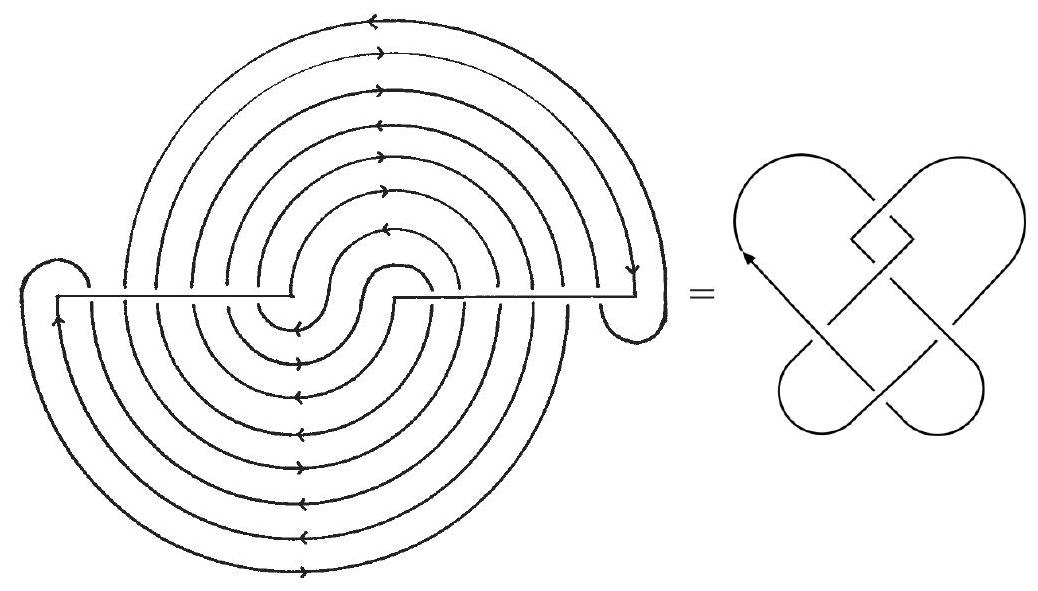
\includegraphics[scale=0.2]{2025_05_21_9c06be8de7a55410f8c1g-052}
\end{center}

Figure 3.6. $\mathfrak{b}(7,3)=5_{2}$.\\
respectively. It follows that $\mathfrak{A}_{n} \neq \varphi\left(\mathfrak{B}_{n}\right)$ and $\psi\left(\mathfrak{B}_{n}\right) \neq \mathfrak{A}_{n+1}$. Proof as E 3.5 (b). A consequence is that the complement of this knot cannot be fibered over $S^{1}$ with a surface as fiber, see Theorem 5.1. This knot also has genus one, i.e. it bounds a torus with one hole.
\end{EXA}




The background to the calculations in Examples 3.8 and 3.9 is discussed in Chapter 4 . The next proposition shows that the fundamental group of the complement characterizes the trivial knot:\\




3.10 Proposition. 


\begin{PROP}{KNO-B14-03-04}{Fundamentalgruppe des Komplements von tabularen Umgebungen charakterisiert den trivialen Knoten}
If $\mathfrak{k}$ is a non-trivial knot the inclusion $i: \partial V \rightarrow C=\overline{S^{3}-V}$ induces an injective homomorphism $i_{\#}: \pi_{1} \partial V \rightarrow \pi_{1} C$. In particular, if $\pi_{1} C \cong \mathbb{Z}$ is cyclic then the knot $\mathfrak{k}$ is trivial.
\end{PROP}

Proof. 

\begin{PROOF}{KNO-B14-03-05}{P: Fundamentalgruppe des Komplements von tabularen Umgebungen charakterisiert den trivialen Knoten}
Suppose $i_{\#}$ is not injective. Then the Loop Theorem of Papakyriakopoulos [281], see Appendix B.5 [159, 4.2], guarantees the existence of a simple closed curve $\kappa$ on $\partial V$ and a disk $\delta$ in $C$ such that
$$
\kappa = \partial \delta 
\quad \text{(hence } \kappa \simeq 0 \text{ in } C\text{),} \quad 
\delta \cap V = \kappa \quad \text{and} \quad 
\kappa \not\simeq 0 \text{ in } \partial V\text{.}
$$
Since $\kappa$ is simple and $\kappa \sim 0$ in $C$ it is a longitude, see 3.2. So there is an annulus $A \subset V$ such that $A \cap \partial V=\kappa, \partial A=\kappa \cup \mathfrak{k}$, as has been shown in Theorem 3.1. This proves that $\mathfrak{k}$ bounds a disk in $S^{3}$ and, hence, is the trivial knot.
\end{PROOF}



\pagebreak



3.11 Groups of satellites and companions. 


Recall the notation of Definition 2.8: $\widetilde{V}$ is an unknotted solid torus in a 3-sphere $\widetilde{S}^{3}$ and $\widetilde{\mathfrak{F}} \subset \widetilde{V}$ a knot such that a meridian of $\widetilde{V}$ is not contractible in $\widetilde{V}-\widetilde{\mathfrak{k}}$. As, by definition, a companion $\widehat{\mathfrak{k}}$ is non-trivial the\\
homomorphisms $i_{\#}: \pi_{1} \partial \widehat{V} \rightarrow \pi_{1}(\widehat{V}-\widehat{\mathfrak{k}}), j_{\#}: \pi_{1} \partial V \rightarrow \pi_{1}\left(\overline{S^{3}-\widehat{V}}\right)$ are injective, see Proposition 3.10 and E 2.9. By the Seifert-van Kampen Theorem we get:\\
3.12 Proposition. With the above notation:

$$
\mathfrak{G}=\pi_{1}\left(S^{3}-\mathfrak{k}\right)=\pi_{1}(\widetilde{V}-\widetilde{\mathfrak{F}}) *_{\pi_{1} \partial \widehat{V}} \pi_{1}\left(S^{3}-\widehat{\mathfrak{k}}\right)=\mathfrak{H} *_{\langle\widehat{t}, \widehat{\lambda}\rangle} \widehat{\mathfrak{F}},
$$

is a free product with amalgamation. Here $\widehat{\widehat{G}}$ is the knot group of the companion knot $\widehat{\mathfrak{k}}, \widehat{t}$ and $\widehat{\lambda}$ represent meridian and longitude of $\widehat{\mathfrak{k}}$ and $\mathfrak{H}=\pi_{1}(\widetilde{V}-\widetilde{\mathfrak{k}})$.

Remark. A satellite is never trivial.\\
3.13 Proposition (Longitude). The longitude $\ell$ of a knot $\mathfrak{k}$ represents an element of the second commutator group of the knot group $\mathfrak{F}$ :

$$
\ell \in \mathbb{F}^{(2)}=\mathbb{G}^{\prime \prime} .
$$

Proof. Consider a Seifert surface $S$ spanning the knot $\mathfrak{k}$ such that for some regular neighborhood $V$ of $\mathfrak{k}$ the intersection $S \cap V$ is an annulus $A$ with $\partial A=\mathfrak{k} \cup \ell$. Thus $\ell=\partial(S-A)$ implies that $\ell \sim 0$ in $C=\overline{S^{3}-V}$. A 1-cycle $z$ of $C$ and $S$ have intersection number $r$ if $z \sim r \cdot m$ in $C$ where $m$ is a meridian of $\mathfrak{k}$. Hence, a curve $\zeta$ represents an element of the commutator subgroup $\mathcal{G}^{\prime}$ if and only if its intersection number with $S$ vanishes. Since $S$ is two-sided, each curve on $S$ can be pushed into $C-S$, and thus has intersection number 0 with $S$ and consequently represents an element of $\mathscr{F}^{\prime}$. If $\alpha_{1}, \beta_{1}, \ldots, \alpha_{g}, \beta_{g}$ is a canonical system of curves on $S$ then

$$
\ell \simeq \prod_{n=1}^{g}\left[\alpha_{n}, \beta_{n}\right],
$$

hence, $\ell \in \mathbb{F}^{(2)}$.

Remark. It follows from the proof of Proposition 3.13 that the canonical homomorphism $\mathfrak{G} \rightarrow \mathbb{Z}$ which maps the meridian to 1 is given by $\gamma \mapsto \operatorname{lk}(\gamma, \mathfrak{k})$. Hence each Wirtinger generator is mapped to 1 .

In what follows we will fix the orientation of $S^{3}$ such that the

$$
\operatorname{lk}(\square)=1 .
$$

3.14 Remark. The longitude $\ell$ of a knot $\mathfrak{F}$ can be read off a regular projection as a word in the Wirtinger generators as follows: run through the knot projection starting on the arc assigned to the generator $s_{k}$. Write down $s_{i}$ (or $s_{i}^{-1}$ ) when undercrossing the arc from right to left (or from left to right) corresponding to $s_{i}$. Add $s_{k}^{\alpha}$ such that the sum of all exponents equals 0. See Figure 3.7, $\mathfrak{k}=5_{2}, k=1, \alpha=5$.\\
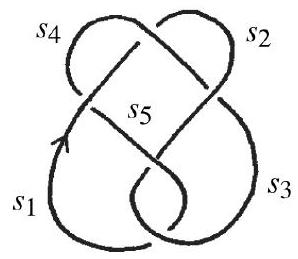
\includegraphics[scale=0.2, center]{2025_05_21_9c06be8de7a55410f8c1g-054}

Figure 3.7 $\ell=s_{4}^{-1} s_{5}^{-1} s_{2}^{-1} s_{1}^{-1} s_{3}^{-1} \cdot s_{1}^{5}$.

\section*{C Peripheral system}
In Paragraph 3.2 we assigned meridian and longitude to a given knot $\mathfrak{k}$. They define homotopy classes in the knot group. These elements are, however, not uniquely determined, but only up to a common conjugating factor. Meridian and longitude can be chosen as free Abelian generators of $\pi_{1} \partial V$. (In this section $C=C(\mathfrak{k})$ always stands for the compact manifold $C=\overline{S^{3}-V}$.)\\
3.15 Definition and Proposition (Peripheral system). The peripheral system of a knot $\mathfrak{k}$ is a triple ( $\mathfrak{G}, m, \ell$ ) consisting of the knot group $\mathfrak{G}$ and the homotopy classes $m, \ell$ of a meridian and a longitude. These elements commute: $m \cdot \ell=\ell \cdot m$. The pair $(m, \ell)$ is uniquely determined up to a common conjugating element of ( $\xi$ ).

The peripheral group system ( $\mathfrak{G}, \mathfrak{B}$ ) consists of $\mathfrak{G}$ and the subgroup $\mathfrak{B}$ generated by $m$ and $\ell, \Re=\pi_{1} \partial V$. As before, the inclusion $\partial V \subset C$ only defines a class of conjugate subgroups $\mathfrak{B}$ of (f).

Theorem 3.16 shows the strength of the peripheral system; unfortunately, its proof depends on a fundamental theorem of F. Waldhausen [367] on 3-manifolds which we cannot prove here.\\[0pt]
3.16 Theorem (Waldhausen [367]). Two knots $\mathfrak{k}_{1}, \mathfrak{k}_{2}$ in $S^{3}$ with the peripheral systems $\left(\mathscr{F}_{i}, m_{i}, \ell_{i}\right), i=1,2$, are equal if there is an isomorphism $\varphi: \mathscr{F}_{1} \rightarrow \mathscr{G}_{2}$ with the property that $\varphi\left(m_{1}\right)=m_{2}$ and $\varphi\left(\ell_{1}\right)=\ell_{2}$.

Proof. Clearly, if $h: S^{3} \rightarrow S^{3}$ is an orientation preserving homeomorphism such that $h\left(\mathfrak{k}_{1}\right)=\mathfrak{k}_{2}$, then the restriction of $h$ to $S^{3}-\mathfrak{k}_{1}$ induces an isomorphism $\varphi: \mathscr{F}_{1} \rightarrow \mathscr{F}_{2}$ satisfying $\varphi\left(m_{1}\right)=m_{2}$ and $\varphi\left(\ell_{1}\right)=\ell_{2}$.

Conversely, assume that $\varphi: \mathfrak{F}_{1} \rightarrow \mathfrak{F}_{2}$ is an isomorphism with the property that $\varphi\left(m_{1}\right)=m_{2}$ and $\varphi\left(\ell_{1}\right)=\ell_{2}$. By the theorem of Waldhausen on sufficiently large irreducible 3-manifolds, see Appendix B. 7 [367, Cor. 6.5], [159, 13.6] the isomorphism $\varphi$ is induced by a homeomorphism $h^{\prime}: C_{1} \rightarrow C_{2}$ mapping representative curves $\mu_{1}, \lambda_{1}$ of $m_{1}, \ell_{1}$ onto representatives $\mu_{2}, \lambda_{2}$ of $m_{2}, \ell_{2}$. The representatives can be taken on the boundaries $\partial C_{i}$. Note that Waldhausen's Theorem B. 7 can be applied in our situation, see Remark B.8.


\end{document}